\documentclass[t]{beamer}

\usepackage{tikz}

\usetikzlibrary{arrows.meta}

\begin{document}
	% CNN
	\begin{frame}[t]
		\vspace{2.5cm}
		\begin{center}
			\begin{figure}[t]
				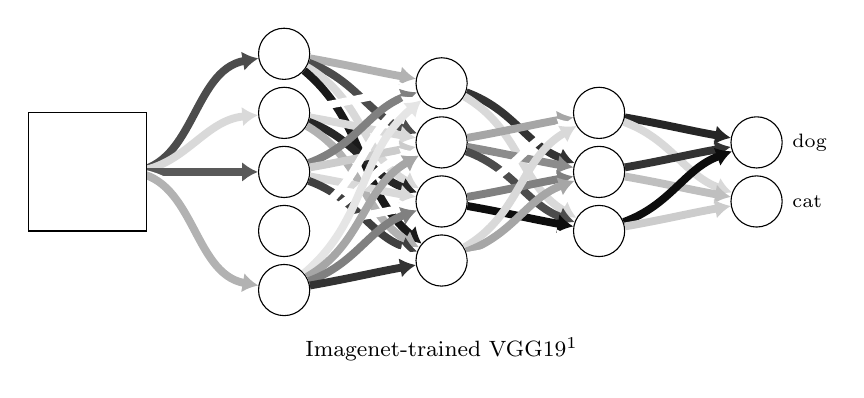
\begin{tikzpicture}
					\node[] at (4.5, -2.25) {\footnotesize{Imagenet-trained VGG19\textsuperscript{1}}};
					\node[circle,draw=black, fill=white, minimum size=0.65cm, inner sep=2pt] (n00) at (2.5,1.5) {};
					\node[circle,draw=black, fill=white, minimum size=0.65cm, inner sep=2pt] (n01) at (2.5,0.75) {};
					\node[circle,draw=black, fill=white, minimum size=0.65cm, inner sep=2pt] (n02) at (2.5,0) {};
					\node[circle,draw=black, fill=white, minimum size=0.65cm, inner sep=2pt] (n03) at (2.5,-0.75) {};
					\node[circle,draw=black, fill=white, minimum size=0.65cm, inner sep=2pt] (n04) at (2.5,-1.5) {};
					
					\node[circle,draw=black, fill=white, minimum size=0.65cm, inner sep=2pt] (n10) at (4.5,1.125) {};
					\node[circle,draw=black, fill=white, minimum size=0.65cm, inner sep=2pt] (n11) at (4.5,0.375) {};
					\node[circle,draw=black, fill=white, minimum size=0.65cm, inner sep=2pt] (n12) at (4.5,-0.375) {};
					\node[circle,draw=black, fill=white, minimum size=0.65cm, inner sep=2pt] (n13) at (4.5,-1.125) {};
					
					\node[circle,draw=black, fill=white, minimum size=0.65cm, inner sep=2pt] (n20) at (6.5,0.75) {};
					\node[circle,draw=black, fill=white, minimum size=0.65cm, inner sep=2pt] (n21) at (6.5,0) {};
					\node[circle,draw=black, fill=white, minimum size=0.65cm, inner sep=2pt] (n22) at (6.5,-0.75) {};
					
					\node[circle,draw=black!, fill=white, minimum size=0.65cm, inner sep=2pt, label=right:{\scriptsize{dog}}] (n31) at (8.5,0.375) {};
					\node[circle,draw=black, fill=white, minimum size=0.65cm, inner sep=2pt, label=right:{\scriptsize{cat}}] (n32) at (8.5,-0.375) {};
					
					\draw[color=black!70,-{Latex[length=0.2cm, width=0.25cm]},line width=0.1cm] (0.5,0) to [out=0,in=190] (n00) {};
					\draw[color=black!15,-{Latex[length=0.2cm, width=0.25cm]},line width=0.1cm] (0.5,0) to [out=0,in=185] (n01) {};
					\draw[color=black!65,-{Latex[length=0.2cm, width=0.25cm]},line width=0.1cm] (0.5,0) to [out=0,in=180] (n02) {};
					\draw[color=white,-{Latex[length=0.2cm, width=0.25cm]},line width=0.1cm] (0.5,0) to [out=0,in=175] (n03) {};
					\draw[color=black!30,-{Latex[length=0.2cm, width=0.25cm]},line width=0.1cm] (0.5,0) to [out=0,in=170] (n04) {};
					
					\node[minimum width=1.5cm, minimum height=1.5cm, inner sep=0pt, draw=black, fill=white] at (0,0) {};
					
					\draw[color=black!30,-{Latex[length=0.2cm, width=0.25cm]},line width=0.1cm] (n00) to [out=-10,in=170] (n10) {};
					\draw[color=black!70,-{Latex[length=0.2cm, width=0.25cm]},line width=0.1cm] (n00) to [out=-20,in=160] (n11) {};
					\draw[color=black!15,-{Latex[length=0.2cm, width=0.25cm]},line width=0.1cm] (n00) to [out=-30,in=150] (n12) {};
					\draw[color=black!90,-{Latex[length=0.2cm, width=0.25cm]},line width=0.1cm] (n00) to [out=-40,in=140] (n13) {};
					
					\draw[color=white,-{Latex[length=0.2cm, width=0.25cm]},line width=0.1cm] (n01) to [out=10,in=190] (n10) {};
					\draw[color=black!15,-{Latex[length=0.2cm, width=0.25cm]},line width=0.1cm] (n01) to [out=-10,in=170] (n11) {};
					\draw[color=black!85,-{Latex[length=0.2cm, width=0.25cm]},line width=0.1cm] (n01) to [out=-20,in=160] (n12) {};
					\draw[color=black!30,-{Latex[length=0.2cm, width=0.25cm]},line width=0.1cm] (n01) to [out=-30,in=150] (n13) {};
					
					\draw[color=black!50,-{Latex[length=0.2cm, width=0.25cm]},line width=0.1cm] (n02) to [out=20,in=200] (n10) {};
					\draw[color=black!20,-{Latex[length=0.2cm, width=0.25cm]},line width=0.1cm] (n02) to [out=10,in=190] (n11) {};
					\draw[color=black!15,-{Latex[length=0.2cm, width=0.25cm]},line width=0.1cm] (n02) to [out=-10,in=170] (n12) {};
					\draw[color=black!75,-{Latex[length=0.2cm, width=0.25cm]},line width=0.1cm] (n02) to [out=-20,in=160] (n13) {};
					
					\draw[color=white,-{Latex[length=0.2cm, width=0.25cm]},line width=0.1cm] (n03) to [out=30,in=210] (n10) {};
					\draw[color=white,-{Latex[length=0.2cm, width=0.25cm]},line width=0.1cm] (n03) to [out=20,in=200] (n11) {};
					\draw[color=white,-{Latex[length=0.2cm, width=0.25cm]},line width=0.1cm] (n03) to [out=10,in=190] (n12) {};
					\draw[color=white,-{Latex[length=0.2cm, width=0.25cm]},line width=0.1cm] (n03) to [out=-10,in=170] (n13) {};
					
					\draw[color=black!10,-{Latex[length=0.2cm, width=0.25cm]},line width=0.1cm] (n04) to [out=40,in=220] (n10) {};
					\draw[color=black!35,-{Latex[length=0.2cm, width=0.25cm]},line width=0.1cm] (n04) to [out=30,in=210] (n11) {};
					\draw[color=black!50,-{Latex[length=0.2cm, width=0.25cm]},line width=0.1cm] (n04) to [out=20,in=200] (n12) {};
					\draw[color=black!80,-{Latex[length=0.2cm, width=0.25cm]},line width=0.1cm] (n04) to [out=10,in=190] (n13) {};
					
					\draw[color=white,-{Latex[length=0.2cm, width=0.25cm]},line width=0.1cm] (n10) to [out=-10,in=170] (n20) {};
					\draw[color=black!80,-{Latex[length=0.2cm, width=0.25cm]},line width=0.1cm] (n10) to [out=-20,in=160] (n21) {};
					\draw[color=black!15,-{Latex[length=0.2cm, width=0.25cm]},line width=0.1cm] (n10) to [out=-30,in=150] (n22) {};
					
					\draw[color=black!35,-{Latex[length=0.2cm, width=0.25cm]},line width=0.1cm] (n11) to [out=10,in=190] (n20) {};
					\draw[color=black!45,-{Latex[length=0.2cm, width=0.25cm]},line width=0.1cm] (n11) to [out=-10,in=170] (n21) {};
					\draw[color=black!70,-{Latex[length=0.2cm, width=0.25cm]},line width=0.1cm] (n11) to [out=-20,in=160] (n22) {};
					
					\draw[color=white,-{Latex[length=0.2cm, width=0.25cm]},line width=0.1cm] (n12) to [out=20,in=200] (n20) {};
					\draw[color=black!50,-{Latex[length=0.2cm, width=0.25cm]},line width=0.1cm] (n12) to [out=10,in=190] (n21) {};
					\draw[color=black!95,-{Latex[length=0.2cm, width=0.25cm]},line width=0.1cm] (n12) to [out=-10,in=170] (n22) {};
					
					\draw[color=black!15,-{Latex[length=0.2cm, width=0.25cm]},line width=0.1cm] (n13) to [out=30,in=210] (n20) {};
					\draw[color=black!35,-{Latex[length=0.2cm, width=0.25cm]},line width=0.1cm] (n13) to [out=20,in=200] (n21) {};
					\draw[color=white,-{Latex[length=0.2cm, width=0.25cm]},line width=0.1cm] (n13) to [out=10,in=190] (n22) {};
					
					\draw[color=black!85,-{Latex[length=0.2cm, width=0.25cm]},line width=0.1cm] (n20) to [out=-10,in=170] (n31) {};
					\draw[color=black!15,-{Latex[length=0.2cm, width=0.25cm]},line width=0.1cm] (n20) to [out=-20,in=160] (n32) {};
					
					\draw[color=black!80,-{Latex[length=0.2cm, width=0.25cm]},line width=0.1cm] (n21) to [out=10,in=190] (n31) {};
					\draw[color=black!25,-{Latex[length=0.2cm, width=0.25cm]},line width=0.1cm] (n21) to [out=-10,in=170] (n32) {};
					
					\draw[color=black!95,-{Latex[length=0.2cm, width=0.25cm]},line width=0.1cm] (n22) to [out=20,in=200] (n31) {};
					\draw[color=black!20,-{Latex[length=0.2cm, width=0.25cm]},line width=0.1cm] (n22) to [out=10,in=190] (n32) {};
					
				\end{tikzpicture}
			\end{figure}
		\end{center}
	\end{frame}
	
	% CNN forward pass 1/5
	\begin{frame}[t]
		\vspace{2.5cm}
		\begin{center}
			\begin{figure}[t]
				\begin{tikzpicture}
					\node[circle,draw=black, fill=white, minimum size=0.65cm, inner sep=2pt] (n00) at (2.5,1.5) {};
					\node[circle,draw=black, fill=white, minimum size=0.65cm, inner sep=2pt] (n01) at (2.5,0.75) {};
					\node[circle,draw=black, fill=white, minimum size=0.65cm, inner sep=2pt] (n02) at (2.5,0) {};
					\node[circle,draw=black, fill=white, minimum size=0.65cm, inner sep=2pt] (n03) at (2.5,-0.75) {};
					\node[circle,draw=black, fill=white, minimum size=0.65cm, inner sep=2pt] (n04) at (2.5,-1.5) {};
					
					\node[circle,draw=black, fill=white, minimum size=0.65cm, inner sep=2pt] (n10) at (4.5,1.125) {};
					\node[circle,draw=black, fill=white, minimum size=0.65cm, inner sep=2pt] (n11) at (4.5,0.375) {};
					\node[circle,draw=black, fill=white, minimum size=0.65cm, inner sep=2pt] (n12) at (4.5,-0.375) {};
					\node[circle,draw=black, fill=white, minimum size=0.65cm, inner sep=2pt] (n13) at (4.5,-1.125) {};
					
					\node[circle,draw=black, fill=white, minimum size=0.65cm, inner sep=2pt] (n20) at (6.5,0.75) {};
					\node[circle,draw=black, fill=white, minimum size=0.65cm, inner sep=2pt] (n21) at (6.5,0) {};
					\node[circle,draw=black, fill=white, minimum size=0.65cm, inner sep=2pt] (n22) at (6.5,-0.75) {};
					
					\node[circle,draw=black!, fill=white, minimum size=0.65cm, inner sep=2pt, label=right:{\scriptsize{dog}}] (n31) at (8.5,0.375) {};
					\node[circle,draw=black, fill=white, minimum size=0.65cm, inner sep=2pt, label=right:{\scriptsize{cat}}] (n32) at (8.5,-0.375) {};
					
					\draw[color=black!70,-{Latex[length=0.2cm, width=0.25cm]},line width=0.1cm] (0.5,0) to [out=0,in=190] (n00) {};
					\draw[color=black!15,-{Latex[length=0.2cm, width=0.25cm]},line width=0.1cm] (0.5,0) to [out=0,in=185] (n01) {};
					\draw[color=black!65,-{Latex[length=0.2cm, width=0.25cm]},line width=0.1cm] (0.5,0) to [out=0,in=180] (n02) {};
					\draw[color=white,-{Latex[length=0.2cm, width=0.25cm]},line width=0.1cm] (0.5,0) to [out=0,in=175] (n03) {};
					\draw[color=black!30,-{Latex[length=0.2cm, width=0.25cm]},line width=0.1cm] (0.5,0) to [out=0,in=170] (n04) {};
					
					\node[inner sep=0pt, draw=black] at (0,0) {
						
\includegraphics[width=1.5cm]{data/dog.png}
					};
					
					\draw[color=black!30,-{Latex[length=0.2cm, width=0.25cm]},line width=0.1cm] (n00) to [out=-10,in=170] (n10) {};
					\draw[color=black!70,-{Latex[length=0.2cm, width=0.25cm]},line width=0.1cm] (n00) to [out=-20,in=160] (n11) {};
					\draw[color=black!15,-{Latex[length=0.2cm, width=0.25cm]},line width=0.1cm] (n00) to [out=-30,in=150] (n12) {};
					\draw[color=black!90,-{Latex[length=0.2cm, width=0.25cm]},line width=0.1cm] (n00) to [out=-40,in=140] (n13) {};
					
					\draw[color=white,-{Latex[length=0.2cm, width=0.25cm]},line width=0.1cm] (n01) to [out=10,in=190] (n10) {};
					\draw[color=black!15,-{Latex[length=0.2cm, width=0.25cm]},line width=0.1cm] (n01) to [out=-10,in=170] (n11) {};
					\draw[color=black!85,-{Latex[length=0.2cm, width=0.25cm]},line width=0.1cm] (n01) to [out=-20,in=160] (n12) {};
					\draw[color=black!30,-{Latex[length=0.2cm, width=0.25cm]},line width=0.1cm] (n01) to [out=-30,in=150] (n13) {};
					
					\draw[color=black!50,-{Latex[length=0.2cm, width=0.25cm]},line width=0.1cm] (n02) to [out=20,in=200] (n10) {};
					\draw[color=black!20,-{Latex[length=0.2cm, width=0.25cm]},line width=0.1cm] (n02) to [out=10,in=190] (n11) {};
					\draw[color=black!15,-{Latex[length=0.2cm, width=0.25cm]},line width=0.1cm] (n02) to [out=-10,in=170] (n12) {};
					\draw[color=black!75,-{Latex[length=0.2cm, width=0.25cm]},line width=0.1cm] (n02) to [out=-20,in=160] (n13) {};
					
					\draw[color=white,-{Latex[length=0.2cm, width=0.25cm]},line width=0.1cm] (n03) to [out=30,in=210] (n10) {};
					\draw[color=white,-{Latex[length=0.2cm, width=0.25cm]},line width=0.1cm] (n03) to [out=20,in=200] (n11) {};
					\draw[color=white,-{Latex[length=0.2cm, width=0.25cm]},line width=0.1cm] (n03) to [out=10,in=190] (n12) {};
					\draw[color=white,-{Latex[length=0.2cm, width=0.25cm]},line width=0.1cm] (n03) to [out=-10,in=170] (n13) {};
					
					\draw[color=black!10,-{Latex[length=0.2cm, width=0.25cm]},line width=0.1cm] (n04) to [out=40,in=220] (n10) {};
					\draw[color=black!35,-{Latex[length=0.2cm, width=0.25cm]},line width=0.1cm] (n04) to [out=30,in=210] (n11) {};
					\draw[color=black!50,-{Latex[length=0.2cm, width=0.25cm]},line width=0.1cm] (n04) to [out=20,in=200] (n12) {};
					\draw[color=black!80,-{Latex[length=0.2cm, width=0.25cm]},line width=0.1cm] (n04) to [out=10,in=190] (n13) {};
					
					\draw[color=white,-{Latex[length=0.2cm, width=0.25cm]},line width=0.1cm] (n10) to [out=-10,in=170] (n20) {};
					\draw[color=black!80,-{Latex[length=0.2cm, width=0.25cm]},line width=0.1cm] (n10) to [out=-20,in=160] (n21) {};
					\draw[color=black!15,-{Latex[length=0.2cm, width=0.25cm]},line width=0.1cm] (n10) to [out=-30,in=150] (n22) {};
					
					\draw[color=black!35,-{Latex[length=0.2cm, width=0.25cm]},line width=0.1cm] (n11) to [out=10,in=190] (n20) {};
					\draw[color=black!45,-{Latex[length=0.2cm, width=0.25cm]},line width=0.1cm] (n11) to [out=-10,in=170] (n21) {};
					\draw[color=black!70,-{Latex[length=0.2cm, width=0.25cm]},line width=0.1cm] (n11) to [out=-20,in=160] (n22) {};
					
					\draw[color=white,-{Latex[length=0.2cm, width=0.25cm]},line width=0.1cm] (n12) to [out=20,in=200] (n20) {};
					\draw[color=black!50,-{Latex[length=0.2cm, width=0.25cm]},line width=0.1cm] (n12) to [out=10,in=190] (n21) {};
					\draw[color=black!95,-{Latex[length=0.2cm, width=0.25cm]},line width=0.1cm] (n12) to [out=-10,in=170] (n22) {};
					
					\draw[color=black!15,-{Latex[length=0.2cm, width=0.25cm]},line width=0.1cm] (n13) to [out=30,in=210] (n20) {};
					\draw[color=black!35,-{Latex[length=0.2cm, width=0.25cm]},line width=0.1cm] (n13) to [out=20,in=200] (n21) {};
					\draw[color=white,-{Latex[length=0.2cm, width=0.25cm]},line width=0.1cm] (n13) to [out=10,in=190] (n22) {};
					
					\draw[color=black!85,-{Latex[length=0.2cm, width=0.25cm]},line width=0.1cm] (n20) to [out=-10,in=170] (n31) {};
					\draw[color=black!15,-{Latex[length=0.2cm, width=0.25cm]},line width=0.1cm] (n20) to [out=-20,in=160] (n32) {};
					
					\draw[color=black!80,-{Latex[length=0.2cm, width=0.25cm]},line width=0.1cm] (n21) to [out=10,in=190] (n31) {};
					\draw[color=black!25,-{Latex[length=0.2cm, width=0.25cm]},line width=0.1cm] (n21) to [out=-10,in=170] (n32) {};
					
					\draw[color=black!95,-{Latex[length=0.2cm, width=0.25cm]},line width=0.1cm] (n22) to [out=20,in=200] (n31) {};
					\draw[color=black!20,-{Latex[length=0.2cm, width=0.25cm]},line width=0.1cm] (n22) to [out=10,in=190] (n32) {};
					
				\end{tikzpicture}
			\end{figure}
		\end{center}
	\end{frame}
	
	% CNN forward pass 2/5
	\begin{frame}
		\vspace{2.5cm}
		\begin{center}
			\begin{figure}
				\begin{tikzpicture}
					\node[circle,draw=black!70, fill=black!70, minimum size=0.65cm, inner sep=2pt] (n00) at (2.5,1.5) {\textcolor{white}{\tiny{0.70}}};
					\node[circle,draw=black!15, fill=black!15, minimum size=0.65cm, inner sep=2pt] (n01) at (2.5,0.75) {\tiny{0.15}};
					\node[circle,draw=black!65, fill=black!65, minimum size=0.65cm, inner sep=2pt] (n02) at (2.5,0) {\textcolor{white}{\tiny{0.65}}};
					\node[circle,draw=white, fill=white, minimum size=0.65cm, inner sep=2pt] (n03) at (2.5,-0.75) {};
					\node[circle,draw=black!30, fill=black!30, minimum size=0.65cm, inner sep=2pt] (n04) at (2.5,-1.5) {\tiny{0.30}};
					
					\node[circle,draw=black, fill=white, minimum size=0.65cm, inner sep=2pt] (n10) at (4.5,1.125) {};
					\node[circle,draw=black, fill=white, minimum size=0.65cm, inner sep=2pt] (n11) at (4.5,0.375) {};
					\node[circle,draw=black, fill=white, minimum size=0.65cm, inner sep=2pt] (n12) at (4.5,-0.375) {};
					\node[circle,draw=black, fill=white, minimum size=0.65cm, inner sep=2pt] (n13) at (4.5,-1.125) {};
					
					\node[circle,draw=black, fill=white, minimum size=0.65cm, inner sep=2pt] (n20) at (6.5,0.75) {};
					\node[circle,draw=black, fill=white, minimum size=0.65cm, inner sep=2pt] (n21) at (6.5,0) {};
					\node[circle,draw=black, fill=white, minimum size=0.65cm, inner sep=2pt] (n22) at (6.5,-0.75) {};
					
					\node[circle,draw=black!, fill=white, minimum size=0.65cm, inner sep=2pt, label=right:{\scriptsize{dog}}] (n31) at (8.5,0.375) {};
					\node[circle,draw=black, fill=white, minimum size=0.65cm, inner sep=2pt, label=right:{\scriptsize{cat}}] (n32) at (8.5,-0.375) {};
					
					\draw[color=black!70,-{Latex[length=0.2cm, width=0.25cm]},line width=0.1cm] (0.5,0) to [out=0,in=190] (n00) {};
					\draw[color=black!15,-{Latex[length=0.2cm, width=0.25cm]},line width=0.1cm] (0.5,0) to [out=0,in=185] (n01) {};
					\draw[color=black!65,-{Latex[length=0.2cm, width=0.25cm]},line width=0.1cm] (0.5,0) to [out=0,in=180] (n02) {};
					\draw[color=white,-{Latex[length=0.2cm, width=0.25cm]},line width=0.1cm] (0.5,0) to [out=0,in=175] (n03) {};
					\draw[color=black!30,-{Latex[length=0.2cm, width=0.25cm]},line width=0.1cm] (0.5,0) to [out=0,in=170] (n04) {};
					
					\node[inner sep=0pt, draw=black] at (0,0) {
						
\includegraphics[width=1.5cm]{data/dog.png}
					};
					
					\draw[color=black!30,-{Latex[length=0.2cm, width=0.25cm]},line width=0.1cm] (n00) to [out=-10,in=170] (n10) {};
					\draw[color=black!70,-{Latex[length=0.2cm, width=0.25cm]},line width=0.1cm] (n00) to [out=-20,in=160] (n11) {};
					\draw[color=black!15,-{Latex[length=0.2cm, width=0.25cm]},line width=0.1cm] (n00) to [out=-30,in=150] (n12) {};
					\draw[color=black!90,-{Latex[length=0.2cm, width=0.25cm]},line width=0.1cm] (n00) to [out=-40,in=140] (n13) {};
					
					\draw[color=white,-{Latex[length=0.2cm, width=0.25cm]},line width=0.1cm] (n01) to [out=10,in=190] (n10) {};
					\draw[color=black!15,-{Latex[length=0.2cm, width=0.25cm]},line width=0.1cm] (n01) to [out=-10,in=170] (n11) {};
					\draw[color=black!85,-{Latex[length=0.2cm, width=0.25cm]},line width=0.1cm] (n01) to [out=-20,in=160] (n12) {};
					\draw[color=black!30,-{Latex[length=0.2cm, width=0.25cm]},line width=0.1cm] (n01) to [out=-30,in=150] (n13) {};
					
					\draw[color=black!50,-{Latex[length=0.2cm, width=0.25cm]},line width=0.1cm] (n02) to [out=20,in=200] (n10) {};
					\draw[color=black!20,-{Latex[length=0.2cm, width=0.25cm]},line width=0.1cm] (n02) to [out=10,in=190] (n11) {};
					\draw[color=black!15,-{Latex[length=0.2cm, width=0.25cm]},line width=0.1cm] (n02) to [out=-10,in=170] (n12) {};
					\draw[color=black!75,-{Latex[length=0.2cm, width=0.25cm]},line width=0.1cm] (n02) to [out=-20,in=160] (n13) {};
					
					\draw[color=white,-{Latex[length=0.2cm, width=0.25cm]},line width=0.1cm] (n03) to [out=30,in=210] (n10) {};
					\draw[color=white,-{Latex[length=0.2cm, width=0.25cm]},line width=0.1cm] (n03) to [out=20,in=200] (n11) {};
					\draw[color=white,-{Latex[length=0.2cm, width=0.25cm]},line width=0.1cm] (n03) to [out=10,in=190] (n12) {};
					\draw[color=white,-{Latex[length=0.2cm, width=0.25cm]},line width=0.1cm] (n03) to [out=-10,in=170] (n13) {};
					
					\draw[color=black!10,-{Latex[length=0.2cm, width=0.25cm]},line width=0.1cm] (n04) to [out=40,in=220] (n10) {};
					\draw[color=black!35,-{Latex[length=0.2cm, width=0.25cm]},line width=0.1cm] (n04) to [out=30,in=210] (n11) {};
					\draw[color=black!50,-{Latex[length=0.2cm, width=0.25cm]},line width=0.1cm] (n04) to [out=20,in=200] (n12) {};
					\draw[color=black!80,-{Latex[length=0.2cm, width=0.25cm]},line width=0.1cm] (n04) to [out=10,in=190] (n13) {};
					
					\draw[color=white,-{Latex[length=0.2cm, width=0.25cm]},line width=0.1cm] (n10) to [out=-10,in=170] (n20) {};
					\draw[color=black!80,-{Latex[length=0.2cm, width=0.25cm]},line width=0.1cm] (n10) to [out=-20,in=160] (n21) {};
					\draw[color=black!15,-{Latex[length=0.2cm, width=0.25cm]},line width=0.1cm] (n10) to [out=-30,in=150] (n22) {};
					
					\draw[color=black!35,-{Latex[length=0.2cm, width=0.25cm]},line width=0.1cm] (n11) to [out=10,in=190] (n20) {};
					\draw[color=black!45,-{Latex[length=0.2cm, width=0.25cm]},line width=0.1cm] (n11) to [out=-10,in=170] (n21) {};
					\draw[color=black!70,-{Latex[length=0.2cm, width=0.25cm]},line width=0.1cm] (n11) to [out=-20,in=160] (n22) {};
					
					\draw[color=white,-{Latex[length=0.2cm, width=0.25cm]},line width=0.1cm] (n12) to [out=20,in=200] (n20) {};
					\draw[color=black!50,-{Latex[length=0.2cm, width=0.25cm]},line width=0.1cm] (n12) to [out=10,in=190] (n21) {};
					\draw[color=black!95,-{Latex[length=0.2cm, width=0.25cm]},line width=0.1cm] (n12) to [out=-10,in=170] (n22) {};
					
					\draw[color=black!15,-{Latex[length=0.2cm, width=0.25cm]},line width=0.1cm] (n13) to [out=30,in=210] (n20) {};
					\draw[color=black!35,-{Latex[length=0.2cm, width=0.25cm]},line width=0.1cm] (n13) to [out=20,in=200] (n21) {};
					\draw[color=white,-{Latex[length=0.2cm, width=0.25cm]},line width=0.1cm] (n13) to [out=10,in=190] (n22) {};
					
					\draw[color=black!85,-{Latex[length=0.2cm, width=0.25cm]},line width=0.1cm] (n20) to [out=-10,in=170] (n31) {};
					\draw[color=black!15,-{Latex[length=0.2cm, width=0.25cm]},line width=0.1cm] (n20) to [out=-20,in=160] (n32) {};
					
					\draw[color=black!80,-{Latex[length=0.2cm, width=0.25cm]},line width=0.1cm] (n21) to [out=10,in=190] (n31) {};
					\draw[color=black!25,-{Latex[length=0.2cm, width=0.25cm]},line width=0.1cm] (n21) to [out=-10,in=170] (n32) {};
					
					\draw[color=black!95,-{Latex[length=0.2cm, width=0.25cm]},line width=0.1cm] (n22) to [out=20,in=200] (n31) {};
					\draw[color=black!20,-{Latex[length=0.2cm, width=0.25cm]},line width=0.1cm] (n22) to [out=10,in=190] (n32) {};
					
				\end{tikzpicture}
			\end{figure}
		\end{center}
	\end{frame}
	
	% CNN forward pass 3/5
	\begin{frame}
		\vspace{2.5cm}
		\begin{center}
			\begin{figure}
				\begin{tikzpicture}
					\node[circle,draw=black!70, fill=black!70, minimum size=0.65cm, inner sep=2pt] (n00) at (2.5,1.5) {\textcolor{white}{\tiny{0.70}}};
					\node[circle,draw=black!15, fill=black!15, minimum size=0.65cm, inner sep=2pt] (n01) at (2.5,0.75) {\tiny{0.15}};
					\node[circle,draw=black!65, fill=black!65, minimum size=0.65cm, inner sep=2pt] (n02) at (2.5,0) {\textcolor{white}{\tiny{0.65}}};
					\node[circle,draw=white, fill=white, minimum size=0.65cm, inner sep=2pt] (n03) at (2.5,-0.75) {};
					\node[circle,draw=black!30, fill=black!30, minimum size=0.65cm, inner sep=2pt] (n04) at (2.5,-1.5) {\tiny{0.30}};
					
					\node[circle,draw=black!35, fill=black!35, minimum size=0.65cm, inner sep=2pt] (n10) at (4.5,1.125) {\tiny{0.35}};
					\node[circle,draw=black!20, fill=black!20, minimum size=0.65cm, inner sep=2pt] (n11) at (4.5,0.375) {\tiny{0.20}};
					\node[circle,draw=black!40, fill=black!40, minimum size=0.65cm, inner sep=2pt] (n12) at (4.5,-0.375) {\tiny{0.40}};
					\node[circle,draw=black!85, fill=black!85, minimum size=0.65cm, inner sep=2pt] (n13) at (4.5,-1.125) {\textcolor{white}{\tiny{0.85}}};
					
					\node[circle,draw=black, fill=white, minimum size=0.65cm, inner sep=2pt] (n20) at (6.5,0.75) {};
					\node[circle,draw=black, fill=white, minimum size=0.65cm, inner sep=2pt] (n21) at (6.5,0) {};
					\node[circle,draw=black, fill=white, minimum size=0.65cm, inner sep=2pt] (n22) at (6.5,-0.75) {};
					
					\node[circle,draw=black!, fill=white, minimum size=0.65cm, inner sep=2pt, label=right:{\scriptsize{dog}}] (n31) at (8.5,0.375) {};
					\node[circle,draw=black, fill=white, minimum size=0.65cm, inner sep=2pt, label=right:{\scriptsize{cat}}] (n32) at (8.5,-0.375) {};
					
					\draw[color=black!70,-{Latex[length=0.2cm, width=0.25cm]},line width=0.1cm] (0.5,0) to [out=0,in=190] (n00) {};
					\draw[color=black!15,-{Latex[length=0.2cm, width=0.25cm]},line width=0.1cm] (0.5,0) to [out=0,in=185] (n01) {};
					\draw[color=black!65,-{Latex[length=0.2cm, width=0.25cm]},line width=0.1cm] (0.5,0) to [out=0,in=180] (n02) {};
					\draw[color=white,-{Latex[length=0.2cm, width=0.25cm]},line width=0.1cm] (0.5,0) to [out=0,in=175] (n03) {};
					\draw[color=black!30,-{Latex[length=0.2cm, width=0.25cm]},line width=0.1cm] (0.5,0) to [out=0,in=170] (n04) {};
					
					\node[inner sep=0pt, draw=black] at (0,0) {
						
\includegraphics[width=1.5cm]{data/dog.png}
					};
					
					\draw[color=black!30,-{Latex[length=0.2cm, width=0.25cm]},line width=0.1cm] (n00) to [out=-10,in=170] (n10) {};
					\draw[color=black!70,-{Latex[length=0.2cm, width=0.25cm]},line width=0.1cm] (n00) to [out=-20,in=160] (n11) {};
					\draw[color=black!15,-{Latex[length=0.2cm, width=0.25cm]},line width=0.1cm] (n00) to [out=-30,in=150] (n12) {};
					\draw[color=black!90,-{Latex[length=0.2cm, width=0.25cm]},line width=0.1cm] (n00) to [out=-40,in=140] (n13) {};
					
					\draw[color=white,-{Latex[length=0.2cm, width=0.25cm]},line width=0.1cm] (n01) to [out=10,in=190] (n10) {};
					\draw[color=black!15,-{Latex[length=0.2cm, width=0.25cm]},line width=0.1cm] (n01) to [out=-10,in=170] (n11) {};
					\draw[color=black!85,-{Latex[length=0.2cm, width=0.25cm]},line width=0.1cm] (n01) to [out=-20,in=160] (n12) {};
					\draw[color=black!30,-{Latex[length=0.2cm, width=0.25cm]},line width=0.1cm] (n01) to [out=-30,in=150] (n13) {};
					
					\draw[color=black!50,-{Latex[length=0.2cm, width=0.25cm]},line width=0.1cm] (n02) to [out=20,in=200] (n10) {};
					\draw[color=black!20,-{Latex[length=0.2cm, width=0.25cm]},line width=0.1cm] (n02) to [out=10,in=190] (n11) {};
					\draw[color=black!15,-{Latex[length=0.2cm, width=0.25cm]},line width=0.1cm] (n02) to [out=-10,in=170] (n12) {};
					\draw[color=black!75,-{Latex[length=0.2cm, width=0.25cm]},line width=0.1cm] (n02) to [out=-20,in=160] (n13) {};
					
					\draw[color=white,-{Latex[length=0.2cm, width=0.25cm]},line width=0.1cm] (n03) to [out=30,in=210] (n10) {};
					\draw[color=white,-{Latex[length=0.2cm, width=0.25cm]},line width=0.1cm] (n03) to [out=20,in=200] (n11) {};
					\draw[color=white,-{Latex[length=0.2cm, width=0.25cm]},line width=0.1cm] (n03) to [out=10,in=190] (n12) {};
					\draw[color=white,-{Latex[length=0.2cm, width=0.25cm]},line width=0.1cm] (n03) to [out=-10,in=170] (n13) {};
					
					\draw[color=black!10,-{Latex[length=0.2cm, width=0.25cm]},line width=0.1cm] (n04) to [out=40,in=220] (n10) {};
					\draw[color=black!35,-{Latex[length=0.2cm, width=0.25cm]},line width=0.1cm] (n04) to [out=30,in=210] (n11) {};
					\draw[color=black!50,-{Latex[length=0.2cm, width=0.25cm]},line width=0.1cm] (n04) to [out=20,in=200] (n12) {};
					\draw[color=black!80,-{Latex[length=0.2cm, width=0.25cm]},line width=0.1cm] (n04) to [out=10,in=190] (n13) {};
					
					\draw[color=white,-{Latex[length=0.2cm, width=0.25cm]},line width=0.1cm] (n10) to [out=-10,in=170] (n20) {};
					\draw[color=black!80,-{Latex[length=0.2cm, width=0.25cm]},line width=0.1cm] (n10) to [out=-20,in=160] (n21) {};
					\draw[color=black!15,-{Latex[length=0.2cm, width=0.25cm]},line width=0.1cm] (n10) to [out=-30,in=150] (n22) {};
					
					\draw[color=black!35,-{Latex[length=0.2cm, width=0.25cm]},line width=0.1cm] (n11) to [out=10,in=190] (n20) {};
					\draw[color=black!45,-{Latex[length=0.2cm, width=0.25cm]},line width=0.1cm] (n11) to [out=-10,in=170] (n21) {};
					\draw[color=black!70,-{Latex[length=0.2cm, width=0.25cm]},line width=0.1cm] (n11) to [out=-20,in=160] (n22) {};
					
					\draw[color=white,-{Latex[length=0.2cm, width=0.25cm]},line width=0.1cm] (n12) to [out=20,in=200] (n20) {};
					\draw[color=black!50,-{Latex[length=0.2cm, width=0.25cm]},line width=0.1cm] (n12) to [out=10,in=190] (n21) {};
					\draw[color=black!95,-{Latex[length=0.2cm, width=0.25cm]},line width=0.1cm] (n12) to [out=-10,in=170] (n22) {};
					
					\draw[color=black!15,-{Latex[length=0.2cm, width=0.25cm]},line width=0.1cm] (n13) to [out=30,in=210] (n20) {};
					\draw[color=black!35,-{Latex[length=0.2cm, width=0.25cm]},line width=0.1cm] (n13) to [out=20,in=200] (n21) {};
					\draw[color=white,-{Latex[length=0.2cm, width=0.25cm]},line width=0.1cm] (n13) to [out=10,in=190] (n22) {};
					
					\draw[color=black!85,-{Latex[length=0.2cm, width=0.25cm]},line width=0.1cm] (n20) to [out=-10,in=170] (n31) {};
					\draw[color=black!15,-{Latex[length=0.2cm, width=0.25cm]},line width=0.1cm] (n20) to [out=-20,in=160] (n32) {};
					
					\draw[color=black!80,-{Latex[length=0.2cm, width=0.25cm]},line width=0.1cm] (n21) to [out=10,in=190] (n31) {};
					\draw[color=black!25,-{Latex[length=0.2cm, width=0.25cm]},line width=0.1cm] (n21) to [out=-10,in=170] (n32) {};
					
					\draw[color=black!95,-{Latex[length=0.2cm, width=0.25cm]},line width=0.1cm] (n22) to [out=20,in=200] (n31) {};
					\draw[color=black!20,-{Latex[length=0.2cm, width=0.25cm]},line width=0.1cm] (n22) to [out=10,in=190] (n32) {};
					
				\end{tikzpicture}
			\end{figure}
		\end{center}
	\end{frame}
	
	% CNN forward pass 4/5
	\begin{frame}
		\vspace{2.5cm}
		\begin{center}
			\begin{figure}
				\begin{tikzpicture}
					\node[circle,draw=black!70, fill=black!70, minimum size=0.65cm, inner sep=2pt] (n00) at (2.5,1.5) {\textcolor{white}{\tiny{0.70}}};
					\node[circle,draw=black!15, fill=black!15, minimum size=0.65cm, inner sep=2pt] (n01) at (2.5,0.75) {\tiny{0.15}};
					\node[circle,draw=black!65, fill=black!65, minimum size=0.65cm, inner sep=2pt] (n02) at (2.5,0) {\textcolor{white}{\tiny{0.65}}};
					\node[circle,draw=white, fill=white, minimum size=0.65cm, inner sep=2pt] (n03) at (2.5,-0.75) {};
					\node[circle,draw=black!30, fill=black!30, minimum size=0.65cm, inner sep=2pt] (n04) at (2.5,-1.5) {\tiny{0.30}};
					
					\node[circle,draw=black!35, fill=black!35, minimum size=0.65cm, inner sep=2pt] (n10) at (4.5,1.125) {\tiny{0.35}};
					\node[circle,draw=black!20, fill=black!20, minimum size=0.65cm, inner sep=2pt] (n11) at (4.5,0.375) {\tiny{0.20}};
					\node[circle,draw=black!40, fill=black!40, minimum size=0.65cm, inner sep=2pt] (n12) at (4.5,-0.375) {\tiny{0.40}};
					\node[circle,draw=black!85, fill=black!85, minimum size=0.65cm, inner sep=2pt] (n13) at (4.5,-1.125) {\textcolor{white}{\tiny{0.85}}};
					
					\node[circle,draw=black!10, fill=black!10, minimum size=0.65cm, inner sep=2pt] (n20) at (6.5,0.75) {\tiny{0.10}};
					\node[circle,draw=black!95, fill=black!95, minimum size=0.65cm, inner sep=2pt] (n21) at (6.5,0) {\textcolor{white}{\tiny{0.95}}};
					\node[circle,draw=black!70, fill=black!70, minimum size=0.65cm, inner sep=2pt] (n22) at (6.5,-0.75) {\textcolor{white}{\tiny{0.70}}};
					
					\node[circle,draw=black!, fill=white, minimum size=0.65cm, inner sep=2pt, label=right:{\scriptsize{dog}}] (n31) at (8.5,0.375) {};
					\node[circle,draw=black, fill=white, minimum size=0.65cm, inner sep=2pt, label=right:{\scriptsize{cat}}] (n32) at (8.5,-0.375) {};
					
					\draw[color=black!70,-{Latex[length=0.2cm, width=0.25cm]},line width=0.1cm] (0.5,0) to [out=0,in=190] (n00) {};
					\draw[color=black!15,-{Latex[length=0.2cm, width=0.25cm]},line width=0.1cm] (0.5,0) to [out=0,in=185] (n01) {};
					\draw[color=black!65,-{Latex[length=0.2cm, width=0.25cm]},line width=0.1cm] (0.5,0) to [out=0,in=180] (n02) {};
					\draw[color=white,-{Latex[length=0.2cm, width=0.25cm]},line width=0.1cm] (0.5,0) to [out=0,in=175] (n03) {};
					\draw[color=black!30,-{Latex[length=0.2cm, width=0.25cm]},line width=0.1cm] (0.5,0) to [out=0,in=170] (n04) {};
					
					\node[inner sep=0pt, draw=black] at (0,0) {
						
\includegraphics[width=1.5cm]{data/dog.png}
					};
					
					\draw[color=black!30,-{Latex[length=0.2cm, width=0.25cm]},line width=0.1cm] (n00) to [out=-10,in=170] (n10) {};
					\draw[color=black!70,-{Latex[length=0.2cm, width=0.25cm]},line width=0.1cm] (n00) to [out=-20,in=160] (n11) {};
					\draw[color=black!15,-{Latex[length=0.2cm, width=0.25cm]},line width=0.1cm] (n00) to [out=-30,in=150] (n12) {};
					\draw[color=black!90,-{Latex[length=0.2cm, width=0.25cm]},line width=0.1cm] (n00) to [out=-40,in=140] (n13) {};
					
					\draw[color=white,-{Latex[length=0.2cm, width=0.25cm]},line width=0.1cm] (n01) to [out=10,in=190] (n10) {};
					\draw[color=black!15,-{Latex[length=0.2cm, width=0.25cm]},line width=0.1cm] (n01) to [out=-10,in=170] (n11) {};
					\draw[color=black!85,-{Latex[length=0.2cm, width=0.25cm]},line width=0.1cm] (n01) to [out=-20,in=160] (n12) {};
					\draw[color=black!30,-{Latex[length=0.2cm, width=0.25cm]},line width=0.1cm] (n01) to [out=-30,in=150] (n13) {};
					
					\draw[color=black!50,-{Latex[length=0.2cm, width=0.25cm]},line width=0.1cm] (n02) to [out=20,in=200] (n10) {};
					\draw[color=black!20,-{Latex[length=0.2cm, width=0.25cm]},line width=0.1cm] (n02) to [out=10,in=190] (n11) {};
					\draw[color=black!15,-{Latex[length=0.2cm, width=0.25cm]},line width=0.1cm] (n02) to [out=-10,in=170] (n12) {};
					\draw[color=black!75,-{Latex[length=0.2cm, width=0.25cm]},line width=0.1cm] (n02) to [out=-20,in=160] (n13) {};
					
					\draw[color=white,-{Latex[length=0.2cm, width=0.25cm]},line width=0.1cm] (n03) to [out=30,in=210] (n10) {};
					\draw[color=white,-{Latex[length=0.2cm, width=0.25cm]},line width=0.1cm] (n03) to [out=20,in=200] (n11) {};
					\draw[color=white,-{Latex[length=0.2cm, width=0.25cm]},line width=0.1cm] (n03) to [out=10,in=190] (n12) {};
					\draw[color=white,-{Latex[length=0.2cm, width=0.25cm]},line width=0.1cm] (n03) to [out=-10,in=170] (n13) {};
					
					\draw[color=black!10,-{Latex[length=0.2cm, width=0.25cm]},line width=0.1cm] (n04) to [out=40,in=220] (n10) {};
					\draw[color=black!35,-{Latex[length=0.2cm, width=0.25cm]},line width=0.1cm] (n04) to [out=30,in=210] (n11) {};
					\draw[color=black!50,-{Latex[length=0.2cm, width=0.25cm]},line width=0.1cm] (n04) to [out=20,in=200] (n12) {};
					\draw[color=black!80,-{Latex[length=0.2cm, width=0.25cm]},line width=0.1cm] (n04) to [out=10,in=190] (n13) {};
					
					\draw[color=white,-{Latex[length=0.2cm, width=0.25cm]},line width=0.1cm] (n10) to [out=-10,in=170] (n20) {};
					\draw[color=black!80,-{Latex[length=0.2cm, width=0.25cm]},line width=0.1cm] (n10) to [out=-20,in=160] (n21) {};
					\draw[color=black!15,-{Latex[length=0.2cm, width=0.25cm]},line width=0.1cm] (n10) to [out=-30,in=150] (n22) {};
					
					\draw[color=black!35,-{Latex[length=0.2cm, width=0.25cm]},line width=0.1cm] (n11) to [out=10,in=190] (n20) {};
					\draw[color=black!45,-{Latex[length=0.2cm, width=0.25cm]},line width=0.1cm] (n11) to [out=-10,in=170] (n21) {};
					\draw[color=black!70,-{Latex[length=0.2cm, width=0.25cm]},line width=0.1cm] (n11) to [out=-20,in=160] (n22) {};
					
					\draw[color=white,-{Latex[length=0.2cm, width=0.25cm]},line width=0.1cm] (n12) to [out=20,in=200] (n20) {};
					\draw[color=black!50,-{Latex[length=0.2cm, width=0.25cm]},line width=0.1cm] (n12) to [out=10,in=190] (n21) {};
					\draw[color=black!95,-{Latex[length=0.2cm, width=0.25cm]},line width=0.1cm] (n12) to [out=-10,in=170] (n22) {};
					
					\draw[color=black!15,-{Latex[length=0.2cm, width=0.25cm]},line width=0.1cm] (n13) to [out=30,in=210] (n20) {};
					\draw[color=black!35,-{Latex[length=0.2cm, width=0.25cm]},line width=0.1cm] (n13) to [out=20,in=200] (n21) {};
					\draw[color=white,-{Latex[length=0.2cm, width=0.25cm]},line width=0.1cm] (n13) to [out=10,in=190] (n22) {};
					
					\draw[color=black!85,-{Latex[length=0.2cm, width=0.25cm]},line width=0.1cm] (n20) to [out=-10,in=170] (n31) {};
					\draw[color=black!15,-{Latex[length=0.2cm, width=0.25cm]},line width=0.1cm] (n20) to [out=-20,in=160] (n32) {};
					
					\draw[color=black!80,-{Latex[length=0.2cm, width=0.25cm]},line width=0.1cm] (n21) to [out=10,in=190] (n31) {};
					\draw[color=black!25,-{Latex[length=0.2cm, width=0.25cm]},line width=0.1cm] (n21) to [out=-10,in=170] (n32) {};
					
					\draw[color=black!95,-{Latex[length=0.2cm, width=0.25cm]},line width=0.1cm] (n22) to [out=20,in=200] (n31) {};
					\draw[color=black!20,-{Latex[length=0.2cm, width=0.25cm]},line width=0.1cm] (n22) to [out=10,in=190] (n32) {};
					
				\end{tikzpicture}
			\end{figure}
		\end{center}
	\end{frame}

	% CNN forward pass 5/5
	\begin{frame}
		\vspace{2.5cm}
		\begin{center}
			\begin{figure}
				\begin{tikzpicture}
					\node[circle,draw=black!70, fill=black!70, minimum size=0.65cm, inner sep=2pt] (n00) at (2.5,1.5) {\textcolor{white}{\tiny{0.70}}};
					\node[circle,draw=black!15, fill=black!15, minimum size=0.65cm, inner sep=2pt] (n01) at (2.5,0.75) {\tiny{0.15}};
					\node[circle,draw=black!65, fill=black!65, minimum size=0.65cm, inner sep=2pt] (n02) at (2.5,0) {\textcolor{white}{\tiny{0.65}}};
					\node[circle,draw=white, fill=white, minimum size=0.65cm, inner sep=2pt] (n03) at (2.5,-0.75) {};
					\node[circle,draw=black!30, fill=black!30, minimum size=0.65cm, inner sep=2pt] (n04) at (2.5,-1.5) {\tiny{0.30}};
					
					\node[circle,draw=black!35, fill=black!35, minimum size=0.65cm, inner sep=2pt] (n10) at (4.5,1.125) {\tiny{0.35}};
					\node[circle,draw=black!20, fill=black!20, minimum size=0.65cm, inner sep=2pt] (n11) at (4.5,0.375) {\tiny{0.20}};
					\node[circle,draw=black!40, fill=black!40, minimum size=0.65cm, inner sep=2pt] (n12) at (4.5,-0.375) {\tiny{0.40}};
					\node[circle,draw=black!85, fill=black!85, minimum size=0.65cm, inner sep=2pt] (n13) at (4.5,-1.125) {\textcolor{white}{\tiny{0.85}}};
					
					\node[circle,draw=black!10, fill=black!10, minimum size=0.65cm, inner sep=2pt] (n20) at (6.5,0.75) {\tiny{0.10}};
					\node[circle,draw=black!95, fill=black!95, minimum size=0.65cm, inner sep=2pt] (n21) at (6.5,0) {\textcolor{white}{\tiny{0.95}}};
					\node[circle,draw=black!70, fill=black!70, minimum size=0.65cm, inner sep=2pt] (n22) at (6.5,-0.75) {\textcolor{white}{\tiny{0.70}}};
					
					\node[circle,draw=black!95, fill=black!95, minimum size=0.65cm, inner sep=2pt, label=right:{\scriptsize{dog}}] (n31) at (8.5,0.375) {\textcolor{white}{\tiny{0.98}}};
					\node[circle,draw=black!5, fill=black!5, minimum size=0.65cm, inner sep=2pt, label=right:{\scriptsize{cat}}] (n32) at (8.5,-0.375) {\tiny{0.02}};
					
					\draw[color=black!70,-{Latex[length=0.2cm, width=0.25cm]},line width=0.1cm] (0.5,0) to [out=0,in=190] (n00) {};
					\draw[color=black!15,-{Latex[length=0.2cm, width=0.25cm]},line width=0.1cm] (0.5,0) to [out=0,in=185] (n01) {};
					\draw[color=black!65,-{Latex[length=0.2cm, width=0.25cm]},line width=0.1cm] (0.5,0) to [out=0,in=180] (n02) {};
					\draw[color=white,-{Latex[length=0.2cm, width=0.25cm]},line width=0.1cm] (0.5,0) to [out=0,in=175] (n03) {};
					\draw[color=black!30,-{Latex[length=0.2cm, width=0.25cm]},line width=0.1cm] (0.5,0) to [out=0,in=170] (n04) {};
					
					\node[inner sep=0pt, draw=black] at (0,0) {
						
\includegraphics[width=1.5cm]{data/dog.png}
					};
	
					\draw[color=black!30,-{Latex[length=0.2cm, width=0.25cm]},line width=0.1cm] (n00) to [out=-10,in=170] (n10) {};
					\draw[color=black!70,-{Latex[length=0.2cm, width=0.25cm]},line width=0.1cm] (n00) to [out=-20,in=160] (n11) {};
					\draw[color=black!15,-{Latex[length=0.2cm, width=0.25cm]},line width=0.1cm] (n00) to [out=-30,in=150] (n12) {};
					\draw[color=black!90,-{Latex[length=0.2cm, width=0.25cm]},line width=0.1cm] (n00) to [out=-40,in=140] (n13) {};
					
					\draw[color=white,-{Latex[length=0.2cm, width=0.25cm]},line width=0.1cm] (n01) to [out=10,in=190] (n10) {};
					\draw[color=black!15,-{Latex[length=0.2cm, width=0.25cm]},line width=0.1cm] (n01) to [out=-10,in=170] (n11) {};
					\draw[color=black!85,-{Latex[length=0.2cm, width=0.25cm]},line width=0.1cm] (n01) to [out=-20,in=160] (n12) {};
					\draw[color=black!30,-{Latex[length=0.2cm, width=0.25cm]},line width=0.1cm] (n01) to [out=-30,in=150] (n13) {};
					
					\draw[color=black!50,-{Latex[length=0.2cm, width=0.25cm]},line width=0.1cm] (n02) to [out=20,in=200] (n10) {};
					\draw[color=black!20,-{Latex[length=0.2cm, width=0.25cm]},line width=0.1cm] (n02) to [out=10,in=190] (n11) {};
					\draw[color=black!15,-{Latex[length=0.2cm, width=0.25cm]},line width=0.1cm] (n02) to [out=-10,in=170] (n12) {};
					\draw[color=black!75,-{Latex[length=0.2cm, width=0.25cm]},line width=0.1cm] (n02) to [out=-20,in=160] (n13) {};
					
					\draw[color=white,-{Latex[length=0.2cm, width=0.25cm]},line width=0.1cm] (n03) to [out=30,in=210] (n10) {};
					\draw[color=white,-{Latex[length=0.2cm, width=0.25cm]},line width=0.1cm] (n03) to [out=20,in=200] (n11) {};
					\draw[color=white,-{Latex[length=0.2cm, width=0.25cm]},line width=0.1cm] (n03) to [out=10,in=190] (n12) {};
					\draw[color=white,-{Latex[length=0.2cm, width=0.25cm]},line width=0.1cm] (n03) to [out=-10,in=170] (n13) {};
					
					\draw[color=black!10,-{Latex[length=0.2cm, width=0.25cm]},line width=0.1cm] (n04) to [out=40,in=220] (n10) {};
					\draw[color=black!35,-{Latex[length=0.2cm, width=0.25cm]},line width=0.1cm] (n04) to [out=30,in=210] (n11) {};
					\draw[color=black!50,-{Latex[length=0.2cm, width=0.25cm]},line width=0.1cm] (n04) to [out=20,in=200] (n12) {};
					\draw[color=black!80,-{Latex[length=0.2cm, width=0.25cm]},line width=0.1cm] (n04) to [out=10,in=190] (n13) {};
					
					\draw[color=white,-{Latex[length=0.2cm, width=0.25cm]},line width=0.1cm] (n10) to [out=-10,in=170] (n20) {};
					\draw[color=black!80,-{Latex[length=0.2cm, width=0.25cm]},line width=0.1cm] (n10) to [out=-20,in=160] (n21) {};
					\draw[color=black!15,-{Latex[length=0.2cm, width=0.25cm]},line width=0.1cm] (n10) to [out=-30,in=150] (n22) {};
					
					\draw[color=black!35,-{Latex[length=0.2cm, width=0.25cm]},line width=0.1cm] (n11) to [out=10,in=190] (n20) {};
					\draw[color=black!45,-{Latex[length=0.2cm, width=0.25cm]},line width=0.1cm] (n11) to [out=-10,in=170] (n21) {};
					\draw[color=black!70,-{Latex[length=0.2cm, width=0.25cm]},line width=0.1cm] (n11) to [out=-20,in=160] (n22) {};
					
					\draw[color=white,-{Latex[length=0.2cm, width=0.25cm]},line width=0.1cm] (n12) to [out=20,in=200] (n20) {};
					\draw[color=black!50,-{Latex[length=0.2cm, width=0.25cm]},line width=0.1cm] (n12) to [out=10,in=190] (n21) {};
					\draw[color=black!95,-{Latex[length=0.2cm, width=0.25cm]},line width=0.1cm] (n12) to [out=-10,in=170] (n22) {};
					
					\draw[color=black!15,-{Latex[length=0.2cm, width=0.25cm]},line width=0.1cm] (n13) to [out=30,in=210] (n20) {};
					\draw[color=black!35,-{Latex[length=0.2cm, width=0.25cm]},line width=0.1cm] (n13) to [out=20,in=200] (n21) {};
					\draw[color=white,-{Latex[length=0.2cm, width=0.25cm]},line width=0.1cm] (n13) to [out=10,in=190] (n22) {};
					
					\draw[color=black!85,-{Latex[length=0.2cm, width=0.25cm]},line width=0.1cm] (n20) to [out=-10,in=170] (n31) {};
					\draw[color=black!15,-{Latex[length=0.2cm, width=0.25cm]},line width=0.1cm] (n20) to [out=-20,in=160] (n32) {};
					
					\draw[color=black!80,-{Latex[length=0.2cm, width=0.25cm]},line width=0.1cm] (n21) to [out=10,in=190] (n31) {};
					\draw[color=black!25,-{Latex[length=0.2cm, width=0.25cm]},line width=0.1cm] (n21) to [out=-10,in=170] (n32) {};
					
					\draw[color=black!95,-{Latex[length=0.2cm, width=0.25cm]},line width=0.1cm] (n22) to [out=20,in=200] (n31) {};
					\draw[color=black!20,-{Latex[length=0.2cm, width=0.25cm]},line width=0.1cm] (n22) to [out=10,in=190] (n32) {};
					
				\end{tikzpicture}
			\end{figure}
		\end{center}
	\end{frame}
	
	% LRP formula 1/2
	\begin{frame}[c]{ }
		\begin{center}
			\begin{tabular}{c c}
				LRP\textsuperscript{2}:&$R^l_j = \sum\limits_k \frac{a_jw_{jk}}{\sum\limits_{0,j} a_jw_{jk}}R^{(l+1)}_k$\\
			\end{tabular}
		\end{center}
	\end{frame}
	
	% LRP formula 1/2
	\begin{frame}[c]{ }
		\begin{center}
			\begin{tabular}{c c}
				LRP-0:&$R^l_j = \sum\limits_k \frac{a_jw_{jk}}{\sum\limits_{0,j} a_jw_{jk}}R^{(l+1)}_k$\\
				LRP-$\epsilon$:&$R^l_j = \sum\limits_k \frac{a_jw_{jk}}{\sum\limits_{0,j} a_jw_{jk} + sign(a_jw_{jk})*\epsilon}R^{(l+1)}_k$\\
				LRP-$\alpha\beta$:&$R^l_j = \sum\limits_k \alpha\frac{a_jw_{jk}^+}{\sum\limits_{0,j} a_jw_{jk}} - \beta\frac{a_jw_{jk}^-}{\sum\limits_{0,j} a_jw_{jk}} R^{(l+1)}_k$\\
			\end{tabular}
		\end{center}
	\end{frame}

	% LRP dog backward pass 1/5
	\begin{frame}
		\vspace{2.5cm}
		\begin{center}
			\begin{figure}
				\begin{tikzpicture}
					\node[circle,draw=black!70, fill=black!70, minimum size=0.65cm, inner sep=2pt] (n00) at (2.5,1.5) {\textcolor{white}{\tiny{0.70}}};
					\node[circle,draw=black!15, fill=black!15, minimum size=0.65cm, inner sep=2pt] (n01) at (2.5,0.75) {\tiny{0.15}};
					\node[circle,draw=black!65, fill=black!65, minimum size=0.65cm, inner sep=2pt] (n02) at (2.5,0) {\textcolor{white}{\tiny{0.65}}};
					\node[circle,draw=white, fill=white, minimum size=0.65cm, inner sep=2pt] (n03) at (2.5,-0.75) {};
					\node[circle,draw=black!30, fill=black!30, minimum size=0.65cm, inner sep=2pt] (n04) at (2.5,-1.5) {\tiny{0.30}};
					
					\node[circle,draw=black!35, fill=black!35, minimum size=0.65cm, inner sep=2pt] (n10) at (4.5,1.125) {\tiny{0.35}};
					\node[circle,draw=black!20, fill=black!20, minimum size=0.65cm, inner sep=2pt] (n11) at (4.5,0.375) {\tiny{0.20}};
					\node[circle,draw=black!40, fill=black!40, minimum size=0.65cm, inner sep=2pt] (n12) at (4.5,-0.375) {\tiny{0.40}};
					\node[circle,draw=black!85, fill=black!85, minimum size=0.65cm, inner sep=2pt] (n13) at (4.5,-1.125) {\textcolor{white}{\tiny{0.85}}};
					
					\node[circle,draw=black!10, fill=black!10, minimum size=0.65cm, inner sep=2pt] (n20) at (6.5,0.75) {\tiny{0.10}};
					\node[circle,draw=black!95, fill=black!95, minimum size=0.65cm, inner sep=2pt] (n21) at (6.5,0) {\textcolor{white}{\tiny{0.95}}};
					\node[circle,draw=black!70, fill=black!70, minimum size=0.65cm, inner sep=2pt] (n22) at (6.5,-0.75) {\textcolor{white}{\tiny{0.70}}};
					
					\node[circle,draw=red, fill=red, minimum size=0.65cm, inner sep=2pt, label=right:{\scriptsize{dog}}] (n31) at (8.5,0.375) {\textcolor{white}{\tiny{10}}};
					\node[circle,draw=white, fill=white, minimum size=0.65cm, inner sep=2pt] (n32) at (8.5,-0.375) {\textcolor{white}{\tiny{0.02}}};
					
					\draw[color=black!70,-{Latex[length=0.2cm, width=0.25cm]},line width=0.1cm] (0.5,0) to [out=0,in=190] (n00) {};
					\draw[color=black!15,-{Latex[length=0.2cm, width=0.25cm]},line width=0.1cm] (0.5,0) to [out=0,in=185] (n01) {};
					\draw[color=black!65,-{Latex[length=0.2cm, width=0.25cm]},line width=0.1cm] (0.5,0) to [out=0,in=180] (n02) {};
					\draw[color=white,-{Latex[length=0.2cm, width=0.25cm]},line width=0.1cm] (0.5,0) to [out=0,in=175] (n03) {};
					\draw[color=black!30,-{Latex[length=0.2cm, width=0.25cm]},line width=0.1cm] (0.5,0) to [out=0,in=170] (n04) {};
					
					\node[inner sep=0pt, draw=black] at (0,0) {
						
\includegraphics[width=1.5cm]{data/dog.png}
					};
					
					\draw[color=black!30,-{Latex[length=0.2cm, width=0.25cm]},line width=0.1cm] (n00) to [out=-10,in=170] (n10) {};
					\draw[color=black!70,-{Latex[length=0.2cm, width=0.25cm]},line width=0.1cm] (n00) to [out=-20,in=160] (n11) {};
					\draw[color=black!15,-{Latex[length=0.2cm, width=0.25cm]},line width=0.1cm] (n00) to [out=-30,in=150] (n12) {};
					\draw[color=black!90,-{Latex[length=0.2cm, width=0.25cm]},line width=0.1cm] (n00) to [out=-40,in=140] (n13) {};
					
					\draw[color=white,-{Latex[length=0.2cm, width=0.25cm]},line width=0.1cm] (n01) to [out=10,in=190] (n10) {};
					\draw[color=black!15,-{Latex[length=0.2cm, width=0.25cm]},line width=0.1cm] (n01) to [out=-10,in=170] (n11) {};
					\draw[color=black!85,-{Latex[length=0.2cm, width=0.25cm]},line width=0.1cm] (n01) to [out=-20,in=160] (n12) {};
					\draw[color=black!30,-{Latex[length=0.2cm, width=0.25cm]},line width=0.1cm] (n01) to [out=-30,in=150] (n13) {};
					
					\draw[color=black!50,-{Latex[length=0.2cm, width=0.25cm]},line width=0.1cm] (n02) to [out=20,in=200] (n10) {};
					\draw[color=black!20,-{Latex[length=0.2cm, width=0.25cm]},line width=0.1cm] (n02) to [out=10,in=190] (n11) {};
					\draw[color=black!15,-{Latex[length=0.2cm, width=0.25cm]},line width=0.1cm] (n02) to [out=-10,in=170] (n12) {};
					\draw[color=black!75,-{Latex[length=0.2cm, width=0.25cm]},line width=0.1cm] (n02) to [out=-20,in=160] (n13) {};
					
					\draw[color=white,-{Latex[length=0.2cm, width=0.25cm]},line width=0.1cm] (n03) to [out=30,in=210] (n10) {};
					\draw[color=white,-{Latex[length=0.2cm, width=0.25cm]},line width=0.1cm] (n03) to [out=20,in=200] (n11) {};
					\draw[color=white,-{Latex[length=0.2cm, width=0.25cm]},line width=0.1cm] (n03) to [out=10,in=190] (n12) {};
					\draw[color=white,-{Latex[length=0.2cm, width=0.25cm]},line width=0.1cm] (n03) to [out=-10,in=170] (n13) {};
					
					\draw[color=black!10,-{Latex[length=0.2cm, width=0.25cm]},line width=0.1cm] (n04) to [out=40,in=220] (n10) {};
					\draw[color=black!35,-{Latex[length=0.2cm, width=0.25cm]},line width=0.1cm] (n04) to [out=30,in=210] (n11) {};
					\draw[color=black!50,-{Latex[length=0.2cm, width=0.25cm]},line width=0.1cm] (n04) to [out=20,in=200] (n12) {};
					\draw[color=black!80,-{Latex[length=0.2cm, width=0.25cm]},line width=0.1cm] (n04) to [out=10,in=190] (n13) {};
					
					\draw[color=white,-{Latex[length=0.2cm, width=0.25cm]},line width=0.1cm] (n10) to [out=-10,in=170] (n20) {};
					\draw[color=black!80,-{Latex[length=0.2cm, width=0.25cm]},line width=0.1cm] (n10) to [out=-20,in=160] (n21) {};
					\draw[color=black!15,-{Latex[length=0.2cm, width=0.25cm]},line width=0.1cm] (n10) to [out=-30,in=150] (n22) {};
					
					\draw[color=black!35,-{Latex[length=0.2cm, width=0.25cm]},line width=0.1cm] (n11) to [out=10,in=190] (n20) {};
					\draw[color=black!45,-{Latex[length=0.2cm, width=0.25cm]},line width=0.1cm] (n11) to [out=-10,in=170] (n21) {};
					\draw[color=black!70,-{Latex[length=0.2cm, width=0.25cm]},line width=0.1cm] (n11) to [out=-20,in=160] (n22) {};
					
					\draw[color=white,-{Latex[length=0.2cm, width=0.25cm]},line width=0.1cm] (n12) to [out=20,in=200] (n20) {};
					\draw[color=black!50,-{Latex[length=0.2cm, width=0.25cm]},line width=0.1cm] (n12) to [out=10,in=190] (n21) {};
					\draw[color=black!95,-{Latex[length=0.2cm, width=0.25cm]},line width=0.1cm] (n12) to [out=-10,in=170] (n22) {};
					
					\draw[color=black!15,-{Latex[length=0.2cm, width=0.25cm]},line width=0.1cm] (n13) to [out=30,in=210] (n20) {};
					\draw[color=black!35,-{Latex[length=0.2cm, width=0.25cm]},line width=0.1cm] (n13) to [out=20,in=200] (n21) {};
					\draw[color=white,-{Latex[length=0.2cm, width=0.25cm]},line width=0.1cm] (n13) to [out=10,in=190] (n22) {};
					
					\draw[color=black!85,-{Latex[length=0.2cm, width=0.25cm]},line width=0.1cm] (n20) to [out=-10,in=170] (n31) {};
					\draw[color=black!15,-{Latex[length=0.2cm, width=0.25cm]},line width=0.1cm] (n20) to [out=-20,in=160] (n32) {};
					
					\draw[color=black!80,-{Latex[length=0.2cm, width=0.25cm]},line width=0.1cm] (n21) to [out=10,in=190] (n31) {};
					\draw[color=black!25,-{Latex[length=0.2cm, width=0.25cm]},line width=0.1cm] (n21) to [out=-10,in=170] (n32) {};
					
					\draw[color=black!95,-{Latex[length=0.2cm, width=0.25cm]},line width=0.1cm] (n22) to [out=20,in=200] (n31) {};
					\draw[color=black!20,-{Latex[length=0.2cm, width=0.25cm]},line width=0.1cm] (n22) to [out=10,in=190] (n32) {};
					
				\end{tikzpicture}
			\end{figure}
		\end{center}
	\end{frame}
	
	% LRP dog backward pass 2/5
	\begin{frame}
		\vspace{2.5cm}
		\begin{center}
			\begin{figure}
				\begin{tikzpicture}
					\node[circle,draw=black!70, fill=black!70, minimum size=0.65cm, inner sep=2pt] (n00) at (2.5,1.5) {\textcolor{white}{\tiny{0.70}}};
					\node[circle,draw=black!15, fill=black!15, minimum size=0.65cm, inner sep=2pt] (n01) at (2.5,0.75) {\tiny{0.15}};
					\node[circle,draw=black!65, fill=black!65, minimum size=0.65cm, inner sep=2pt] (n02) at (2.5,0) {\textcolor{white}{\tiny{0.65}}};
					\node[circle,draw=white, fill=white, minimum size=0.65cm, inner sep=2pt] (n03) at (2.5,-0.75) {};
					\node[circle,draw=black!30, fill=black!30, minimum size=0.65cm, inner sep=2pt] (n04) at (2.5,-1.5) {\tiny{0.30}};
					
					\node[circle,draw=black!35, fill=black!35, minimum size=0.65cm, inner sep=2pt] (n10) at (4.5,1.125) {\tiny{0.35}};
					\node[circle,draw=black!20, fill=black!20, minimum size=0.65cm, inner sep=2pt] (n11) at (4.5,0.375) {\tiny{0.20}};
					\node[circle,draw=black!40, fill=black!40, minimum size=0.65cm, inner sep=2pt] (n12) at (4.5,-0.375) {\tiny{0.40}};
					\node[circle,draw=black!85, fill=black!85, minimum size=0.65cm, inner sep=2pt] (n13) at (4.5,-1.125) {\textcolor{white}{\tiny{0.85}}};
					
					\node[circle,draw=red!20, fill=red!20, minimum size=0.65cm, inner sep=2pt] (n20) at (6.5,0.75) {\textcolor{white}{\tiny{1.00}}};
					\node[circle,draw=red!95, fill=red!95, minimum size=0.65cm, inner sep=2pt] (n21) at (6.5,0) {\textcolor{white}{\tiny{5.45}}};
					\node[circle,draw=red!70, fill=red!70, minimum size=0.65cm, inner sep=2pt] (n22) at (6.5,-0.75) {\textcolor{white}{\tiny{3.55}}};
					
					\node[circle,draw=red, fill=red, minimum size=0.65cm, inner sep=2pt, label=right:{\scriptsize{dog}}] (n31) at (8.5,0.375) {\textcolor{white}{\tiny{10}}};
					\node[circle,draw=white, fill=white, minimum size=0.65cm, inner sep=2pt] (n32) at (8.5,-0.375) {\textcolor{white}{\tiny{0.02}}};
					
					\draw[color=black!70,-{Latex[length=0.2cm, width=0.25cm]},line width=0.1cm] (0.5,0) to [out=0,in=190] (n00) {};
					\draw[color=black!15,-{Latex[length=0.2cm, width=0.25cm]},line width=0.1cm] (0.5,0) to [out=0,in=185] (n01) {};
					\draw[color=black!65,-{Latex[length=0.2cm, width=0.25cm]},line width=0.1cm] (0.5,0) to [out=0,in=180] (n02) {};
					\draw[color=white,-{Latex[length=0.2cm, width=0.25cm]},line width=0.1cm] (0.5,0) to [out=0,in=175] (n03) {};
					\draw[color=black!30,-{Latex[length=0.2cm, width=0.25cm]},line width=0.1cm] (0.5,0) to [out=0,in=170] (n04) {};
					
					\node[inner sep=0pt, draw=black] at (0,0) {
						
\includegraphics[width=1.5cm]{data/dog.png}
					};
					
					\draw[color=black!30,-{Latex[length=0.2cm, width=0.25cm]},line width=0.1cm] (n00) to [out=-10,in=170] (n10) {};
					\draw[color=black!70,-{Latex[length=0.2cm, width=0.25cm]},line width=0.1cm] (n00) to [out=-20,in=160] (n11) {};
					\draw[color=black!15,-{Latex[length=0.2cm, width=0.25cm]},line width=0.1cm] (n00) to [out=-30,in=150] (n12) {};
					\draw[color=black!90,-{Latex[length=0.2cm, width=0.25cm]},line width=0.1cm] (n00) to [out=-40,in=140] (n13) {};
					
					\draw[color=white,-{Latex[length=0.2cm, width=0.25cm]},line width=0.1cm] (n01) to [out=10,in=190] (n10) {};
					\draw[color=black!15,-{Latex[length=0.2cm, width=0.25cm]},line width=0.1cm] (n01) to [out=-10,in=170] (n11) {};
					\draw[color=black!85,-{Latex[length=0.2cm, width=0.25cm]},line width=0.1cm] (n01) to [out=-20,in=160] (n12) {};
					\draw[color=black!30,-{Latex[length=0.2cm, width=0.25cm]},line width=0.1cm] (n01) to [out=-30,in=150] (n13) {};
					
					\draw[color=black!50,-{Latex[length=0.2cm, width=0.25cm]},line width=0.1cm] (n02) to [out=20,in=200] (n10) {};
					\draw[color=black!20,-{Latex[length=0.2cm, width=0.25cm]},line width=0.1cm] (n02) to [out=10,in=190] (n11) {};
					\draw[color=black!15,-{Latex[length=0.2cm, width=0.25cm]},line width=0.1cm] (n02) to [out=-10,in=170] (n12) {};
					\draw[color=black!75,-{Latex[length=0.2cm, width=0.25cm]},line width=0.1cm] (n02) to [out=-20,in=160] (n13) {};
					
					\draw[color=white,-{Latex[length=0.2cm, width=0.25cm]},line width=0.1cm] (n03) to [out=30,in=210] (n10) {};
					\draw[color=white,-{Latex[length=0.2cm, width=0.25cm]},line width=0.1cm] (n03) to [out=20,in=200] (n11) {};
					\draw[color=white,-{Latex[length=0.2cm, width=0.25cm]},line width=0.1cm] (n03) to [out=10,in=190] (n12) {};
					\draw[color=white,-{Latex[length=0.2cm, width=0.25cm]},line width=0.1cm] (n03) to [out=-10,in=170] (n13) {};
					
					\draw[color=black!10,-{Latex[length=0.2cm, width=0.25cm]},line width=0.1cm] (n04) to [out=40,in=220] (n10) {};
					\draw[color=black!35,-{Latex[length=0.2cm, width=0.25cm]},line width=0.1cm] (n04) to [out=30,in=210] (n11) {};
					\draw[color=black!50,-{Latex[length=0.2cm, width=0.25cm]},line width=0.1cm] (n04) to [out=20,in=200] (n12) {};
					\draw[color=black!80,-{Latex[length=0.2cm, width=0.25cm]},line width=0.1cm] (n04) to [out=10,in=190] (n13) {};
					
					\draw[color=white,-{Latex[length=0.2cm, width=0.25cm]},line width=0.1cm] (n10) to [out=-10,in=170] (n20) {};
					\draw[color=black!80,-{Latex[length=0.2cm, width=0.25cm]},line width=0.1cm] (n10) to [out=-20,in=160] (n21) {};
					\draw[color=black!15,-{Latex[length=0.2cm, width=0.25cm]},line width=0.1cm] (n10) to [out=-30,in=150] (n22) {};
					
					\draw[color=black!35,-{Latex[length=0.2cm, width=0.25cm]},line width=0.1cm] (n11) to [out=10,in=190] (n20) {};
					\draw[color=black!45,-{Latex[length=0.2cm, width=0.25cm]},line width=0.1cm] (n11) to [out=-10,in=170] (n21) {};
					\draw[color=black!70,-{Latex[length=0.2cm, width=0.25cm]},line width=0.1cm] (n11) to [out=-20,in=160] (n22) {};
					
					\draw[color=white,-{Latex[length=0.2cm, width=0.25cm]},line width=0.1cm] (n12) to [out=20,in=200] (n20) {};
					\draw[color=black!50,-{Latex[length=0.2cm, width=0.25cm]},line width=0.1cm] (n12) to [out=10,in=190] (n21) {};
					\draw[color=black!95,-{Latex[length=0.2cm, width=0.25cm]},line width=0.1cm] (n12) to [out=-10,in=170] (n22) {};
					
					\draw[color=black!15,-{Latex[length=0.2cm, width=0.25cm]},line width=0.1cm] (n13) to [out=30,in=210] (n20) {};
					\draw[color=black!35,-{Latex[length=0.2cm, width=0.25cm]},line width=0.1cm] (n13) to [out=20,in=200] (n21) {};
					\draw[color=white,-{Latex[length=0.2cm, width=0.25cm]},line width=0.1cm] (n13) to [out=10,in=190] (n22) {};
					
					\draw[color=red!85,{Latex[length=0.2cm, width=0.25cm]}-,line width=0.1cm] (n20) to [out=-10,in=170] (n31) {};
					
					\draw[color=red!80,{Latex[length=0.2cm, width=0.25cm]}-,line width=0.1cm] (n21) to [out=10,in=190] (n31) {};
					
					\draw[color=red!95,{Latex[length=0.2cm, width=0.25cm]}-,line width=0.1cm] (n22) to [out=20,in=200] (n31) {};
					
				\end{tikzpicture}
			\end{figure}
		\end{center}
	\end{frame}
	
	% LRP dog backward pass 3/5
	\begin{frame}
		\vspace{2.5cm}
		\begin{center}
			\begin{figure}
				\begin{tikzpicture}
					\node[circle,draw=black!70, fill=black!70, minimum size=0.65cm, inner sep=2pt] (n00) at (2.5,1.5) {\textcolor{white}{\tiny{0.70}}};
					\node[circle,draw=black!15, fill=black!15, minimum size=0.65cm, inner sep=2pt] (n01) at (2.5,0.75) {\tiny{0.15}};
					\node[circle,draw=black!65, fill=black!65, minimum size=0.65cm, inner sep=2pt] (n02) at (2.5,0) {\textcolor{white}{\tiny{0.65}}};
					\node[circle,draw=white, fill=white, minimum size=0.65cm, inner sep=2pt] (n03) at (2.5,-0.75) {};
					\node[circle,draw=black!30, fill=black!30, minimum size=0.65cm, inner sep=2pt] (n04) at (2.5,-1.5) {\tiny{0.30}};
					
					\node[circle,draw=red!35, fill=red!35, minimum size=0.65cm, inner sep=2pt] (n10) at (4.5,1.125) {\textcolor{white}{\tiny{2.85}}};
					\node[circle,draw=red!40, fill=red!40, minimum size=0.65cm, inner sep=2pt] (n11) at (4.5,0.375) {\textcolor{white}{\tiny{1.70}}};
					\node[circle,draw=red!50, fill=red!50, minimum size=0.65cm, inner sep=2pt] (n12) at (4.5,-0.375) {\textcolor{white}{\tiny{3.10}}};
					\node[circle,draw=red!35, fill=red!35, minimum size=0.65cm, inner sep=2pt] (n13) at (4.5,-1.125) {\textcolor{white}{\tiny{2.35}}};
					
					\node[circle,draw=red!20, fill=red!20, minimum size=0.65cm, inner sep=2pt] (n20) at (6.5,0.75) {\textcolor{white}{\tiny{1.00}}};
					\node[circle,draw=red!95, fill=red!95, minimum size=0.65cm, inner sep=2pt] (n21) at (6.5,0) {\textcolor{white}{\tiny{5.45}}};
					\node[circle,draw=red!70, fill=red!70, minimum size=0.65cm, inner sep=2pt] (n22) at (6.5,-0.75) {\textcolor{white}{\tiny{3.55}}};
					
					\node[circle,draw=red, fill=red, minimum size=0.65cm, inner sep=2pt, label=right:{\scriptsize{dog}}] (n31) at (8.5,0.375) {\textcolor{white}{\tiny{10}}};
					\node[circle,draw=white, fill=white, minimum size=0.65cm, inner sep=2pt] (n32) at (8.5,-0.375) {\textcolor{white}{\tiny{0.02}}};
					
					\draw[color=black!70,-{Latex[length=0.2cm, width=0.25cm]},line width=0.1cm] (0.5,0) to [out=0,in=190] (n00) {};
					\draw[color=black!15,-{Latex[length=0.2cm, width=0.25cm]},line width=0.1cm] (0.5,0) to [out=0,in=185] (n01) {};
					\draw[color=black!65,-{Latex[length=0.2cm, width=0.25cm]},line width=0.1cm] (0.5,0) to [out=0,in=180] (n02) {};
					\draw[color=white,-{Latex[length=0.2cm, width=0.25cm]},line width=0.1cm] (0.5,0) to [out=0,in=175] (n03) {};
					\draw[color=black!30,-{Latex[length=0.2cm, width=0.25cm]},line width=0.1cm] (0.5,0) to [out=0,in=170] (n04) {};
					
					\node[inner sep=0pt, draw=black] at (0,0) {
						
\includegraphics[width=1.5cm]{data/dog.png}
					};
					
					\draw[color=black!30,-{Latex[length=0.2cm, width=0.25cm]},line width=0.1cm] (n00) to [out=-10,in=170] (n10) {};
					\draw[color=black!70,-{Latex[length=0.2cm, width=0.25cm]},line width=0.1cm] (n00) to [out=-20,in=160] (n11) {};
					\draw[color=black!15,-{Latex[length=0.2cm, width=0.25cm]},line width=0.1cm] (n00) to [out=-30,in=150] (n12) {};
					\draw[color=black!90,-{Latex[length=0.2cm, width=0.25cm]},line width=0.1cm] (n00) to [out=-40,in=140] (n13) {};
					
					\draw[color=white,-{Latex[length=0.2cm, width=0.25cm]},line width=0.1cm] (n01) to [out=10,in=190] (n10) {};
					\draw[color=black!15,-{Latex[length=0.2cm, width=0.25cm]},line width=0.1cm] (n01) to [out=-10,in=170] (n11) {};
					\draw[color=black!85,-{Latex[length=0.2cm, width=0.25cm]},line width=0.1cm] (n01) to [out=-20,in=160] (n12) {};
					\draw[color=black!30,-{Latex[length=0.2cm, width=0.25cm]},line width=0.1cm] (n01) to [out=-30,in=150] (n13) {};
					
					\draw[color=black!50,-{Latex[length=0.2cm, width=0.25cm]},line width=0.1cm] (n02) to [out=20,in=200] (n10) {};
					\draw[color=black!20,-{Latex[length=0.2cm, width=0.25cm]},line width=0.1cm] (n02) to [out=10,in=190] (n11) {};
					\draw[color=black!15,-{Latex[length=0.2cm, width=0.25cm]},line width=0.1cm] (n02) to [out=-10,in=170] (n12) {};
					\draw[color=black!75,-{Latex[length=0.2cm, width=0.25cm]},line width=0.1cm] (n02) to [out=-20,in=160] (n13) {};
					
					\draw[color=white,-{Latex[length=0.2cm, width=0.25cm]},line width=0.1cm] (n03) to [out=30,in=210] (n10) {};
					\draw[color=white,-{Latex[length=0.2cm, width=0.25cm]},line width=0.1cm] (n03) to [out=20,in=200] (n11) {};
					\draw[color=white,-{Latex[length=0.2cm, width=0.25cm]},line width=0.1cm] (n03) to [out=10,in=190] (n12) {};
					\draw[color=white,-{Latex[length=0.2cm, width=0.25cm]},line width=0.1cm] (n03) to [out=-10,in=170] (n13) {};
					
					\draw[color=black!10,-{Latex[length=0.2cm, width=0.25cm]},line width=0.1cm] (n04) to [out=40,in=220] (n10) {};
					\draw[color=black!35,-{Latex[length=0.2cm, width=0.25cm]},line width=0.1cm] (n04) to [out=30,in=210] (n11) {};
					\draw[color=black!50,-{Latex[length=0.2cm, width=0.25cm]},line width=0.1cm] (n04) to [out=20,in=200] (n12) {};
					\draw[color=black!80,-{Latex[length=0.2cm, width=0.25cm]},line width=0.1cm] (n04) to [out=10,in=190] (n13) {};
					
					\draw[color=white,{Latex[length=0.2cm, width=0.25cm]}-,line width=0.1cm] (n10) to [out=-10,in=170] (n20) {};
					\draw[color=red!80,{Latex[length=0.2cm, width=0.25cm]}-,line width=0.1cm] (n10) to [out=-20,in=160] (n21) {};
					\draw[color=red!15,{Latex[length=0.2cm, width=0.25cm]}-,line width=0.1cm] (n10) to [out=-30,in=150] (n22) {};
					
					\draw[color=red!35,{Latex[length=0.2cm, width=0.25cm]}-,line width=0.1cm] (n11) to [out=10,in=190] (n20) {};
					\draw[color=red!45,{Latex[length=0.2cm, width=0.25cm]}-,line width=0.1cm] (n11) to [out=-10,in=170] (n21) {};
					\draw[color=red!70,{Latex[length=0.2cm, width=0.25cm]}-,line width=0.1cm] (n11) to [out=-20,in=160] (n22) {};
					
					\draw[color=white,{Latex[length=0.2cm, width=0.25cm]}-,line width=0.1cm] (n12) to [out=20,in=200] (n20) {};
					\draw[color=red!50,{Latex[length=0.2cm, width=0.25cm]}-,line width=0.1cm] (n12) to [out=10,in=190] (n21) {};
					\draw[color=red!95,{Latex[length=0.2cm, width=0.25cm]}-,line width=0.1cm] (n12) to [out=-10,in=170] (n22) {};
					
					\draw[color=red!15,{Latex[length=0.2cm, width=0.25cm]}-,line width=0.1cm] (n13) to [out=30,in=210] (n20) {};
					\draw[color=red!35,{Latex[length=0.2cm, width=0.25cm]}-,line width=0.1cm] (n13) to [out=20,in=200] (n21) {};
					\draw[color=white,{Latex[length=0.2cm, width=0.25cm]}-,line width=0.1cm] (n13) to [out=10,in=190] (n22) {};
					
					\draw[color=red!85,{Latex[length=0.2cm, width=0.25cm]}-,line width=0.1cm] (n20) to [out=-10,in=170] (n31) {};
					
					\draw[color=red!80,{Latex[length=0.2cm, width=0.25cm]}-,line width=0.1cm] (n21) to [out=10,in=190] (n31) {};
					
					\draw[color=red!95,{Latex[length=0.2cm, width=0.25cm]}-,line width=0.1cm] (n22) to [out=20,in=200] (n31) {};
					
				\end{tikzpicture}
			\end{figure}
		\end{center}
	\end{frame}

	% LRP dog backward pass 4/5
	\begin{frame}
		\vspace{2.5cm}
		\begin{center}
			\begin{figure}
				\begin{tikzpicture}
					\node[circle,draw=red!70, fill=red!70, minimum size=0.65cm, inner sep=2pt] (n00) at (2.5,1.5) {\textcolor{white}{\tiny{4.25}}};
					\node[circle,draw=white, fill=white, minimum size=0.65cm, inner sep=2pt] (n01) at (2.5,0.75) {};
					\node[circle,draw=red!65, fill=red!65, minimum size=0.65cm, inner sep=2pt] (n02) at (2.5,0) {\textcolor{white}{\tiny{3.90}}};
					\node[circle,draw=white, fill=white, minimum size=0.65cm, inner sep=2pt] (n03) at (2.5,-0.75) {};
					\node[circle,draw=red!30, fill=red!30, minimum size=0.65cm, inner sep=2pt] (n04) at (2.5,-1.5) {\textcolor{white}{\tiny{1.85}}};
					
					\node[circle,draw=red!35, fill=red!35, minimum size=0.65cm, inner sep=2pt] (n10) at (4.5,1.125) {\textcolor{white}{\tiny{2.85}}};
					\node[circle,draw=red!40, fill=red!40, minimum size=0.65cm, inner sep=2pt] (n11) at (4.5,0.375) {\textcolor{white}{\tiny{1.70}}};
					\node[circle,draw=red!50, fill=red!50, minimum size=0.65cm, inner sep=2pt] (n12) at (4.5,-0.375) {\textcolor{white}{\tiny{3.10}}};
					\node[circle,draw=red!35, fill=red!35, minimum size=0.65cm, inner sep=2pt] (n13) at (4.5,-1.125) {\textcolor{white}{\tiny{2.35}}};
					
					\node[circle,draw=red!20, fill=red!20, minimum size=0.65cm, inner sep=2pt] (n20) at (6.5,0.75) {\textcolor{white}{\tiny{1.00}}};
					\node[circle,draw=red!95, fill=red!95, minimum size=0.65cm, inner sep=2pt] (n21) at (6.5,0) {\textcolor{white}{\tiny{5.45}}};
					\node[circle,draw=red!70, fill=red!70, minimum size=0.65cm, inner sep=2pt] (n22) at (6.5,-0.75) {\textcolor{white}{\tiny{3.55}}};
					
					\node[circle,draw=red, fill=red, minimum size=0.65cm, inner sep=2pt, label=right:{\scriptsize{dog}}] (n31) at (8.5,0.375) {\textcolor{white}{\tiny{10}}};
					\node[circle,draw=white, fill=white, minimum size=0.65cm, inner sep=2pt] (n32) at (8.5,-0.375) {\textcolor{white}{\tiny{0.02}}};
					
					\draw[color=black!70,-{Latex[length=0.2cm, width=0.25cm]},line width=0.1cm] (0.5,0) to [out=0,in=190] (n00) {};
					\draw[color=black!15,-{Latex[length=0.2cm, width=0.25cm]},line width=0.1cm] (0.5,0) to [out=0,in=185] (n01) {};
					\draw[color=black!65,-{Latex[length=0.2cm, width=0.25cm]},line width=0.1cm] (0.5,0) to [out=0,in=180] (n02) {};
					\draw[color=white,-{Latex[length=0.2cm, width=0.25cm]},line width=0.1cm] (0.5,0) to [out=0,in=175] (n03) {};
					\draw[color=black!30,-{Latex[length=0.2cm, width=0.25cm]},line width=0.1cm] (0.5,0) to [out=0,in=170] (n04) {};
					
					\node[inner sep=0pt, draw=black] at (0,0) {
						
\includegraphics[width=1.5cm]{data/dog.png}
					};
					
					\draw[color=red!30,{Latex[length=0.2cm, width=0.25cm]}-,line width=0.1cm] (n00) to [out=-10,in=170] (n10) {};
					\draw[color=red!70,{Latex[length=0.2cm, width=0.25cm]}-,line width=0.1cm] (n00) to [out=-20,in=160] (n11) {};
					\draw[color=red!15,{Latex[length=0.2cm, width=0.25cm]}-,line width=0.1cm] (n00) to [out=-30,in=150] (n12) {};
					\draw[color=red!90,{Latex[length=0.2cm, width=0.25cm]}-,line width=0.1cm] (n00) to [out=-40,in=140] (n13) {};
					
					\draw[color=white,{Latex[length=0.2cm, width=0.25cm]}-,line width=0.1cm] (n01) to [out=10,in=190] (n10) {};
					\draw[color=white,{Latex[length=0.2cm, width=0.25cm]}-,line width=0.1cm] (n01) to [out=-10,in=170] (n11) {};
					\draw[color=white,{Latex[length=0.2cm, width=0.25cm]}-,line width=0.1cm] (n01) to [out=-20,in=160] (n12) {};
					\draw[color=white,{Latex[length=0.2cm, width=0.25cm]}-,line width=0.1cm] (n01) to [out=-30,in=150] (n13) {};
					
					\draw[color=red!50,{Latex[length=0.2cm, width=0.25cm]}-,line width=0.1cm] (n02) to [out=20,in=200] (n10) {};
					\draw[color=red!20,{Latex[length=0.2cm, width=0.25cm]}-,line width=0.1cm] (n02) to [out=10,in=190] (n11) {};
					\draw[color=red!15,{Latex[length=0.2cm, width=0.25cm]}-,line width=0.1cm] (n02) to [out=-10,in=170] (n12) {};
					\draw[color=red!75,{Latex[length=0.2cm, width=0.25cm]}-,line width=0.1cm] (n02) to [out=-20,in=160] (n13) {};
					
					\draw[color=white,{Latex[length=0.2cm, width=0.25cm]}-,line width=0.1cm] (n03) to [out=30,in=210] (n10) {};
					\draw[color=white,{Latex[length=0.2cm, width=0.25cm]}-,line width=0.1cm] (n03) to [out=20,in=200] (n11) {};
					\draw[color=white,{Latex[length=0.2cm, width=0.25cm]}-,line width=0.1cm] (n03) to [out=10,in=190] (n12) {};
					\draw[color=white,{Latex[length=0.2cm, width=0.25cm]}-,line width=0.1cm] (n03) to [out=-10,in=170] (n13) {};
					
					\draw[color=red!10,{Latex[length=0.2cm, width=0.25cm]}-,line width=0.1cm] (n04) to [out=40,in=220] (n10) {};
					\draw[color=red!35,{Latex[length=0.2cm, width=0.25cm]}-,line width=0.1cm] (n04) to [out=30,in=210] (n11) {};
					\draw[color=red!50,{Latex[length=0.2cm, width=0.25cm]}-,line width=0.1cm] (n04) to [out=20,in=200] (n12) {};
					\draw[color=red!80,{Latex[length=0.2cm, width=0.25cm]}-,line width=0.1cm] (n04) to [out=10,in=190] (n13) {};
					
					\draw[color=white,{Latex[length=0.2cm, width=0.25cm]}-,line width=0.1cm] (n10) to [out=-10,in=170] (n20) {};
					\draw[color=red!80,{Latex[length=0.2cm, width=0.25cm]}-,line width=0.1cm] (n10) to [out=-20,in=160] (n21) {};
					\draw[color=red!15,{Latex[length=0.2cm, width=0.25cm]}-,line width=0.1cm] (n10) to [out=-30,in=150] (n22) {};
					
					\draw[color=red!35,{Latex[length=0.2cm, width=0.25cm]}-,line width=0.1cm] (n11) to [out=10,in=190] (n20) {};
					\draw[color=red!45,{Latex[length=0.2cm, width=0.25cm]}-,line width=0.1cm] (n11) to [out=-10,in=170] (n21) {};
					\draw[color=red!70,{Latex[length=0.2cm, width=0.25cm]}-,line width=0.1cm] (n11) to [out=-20,in=160] (n22) {};
					
					\draw[color=white,{Latex[length=0.2cm, width=0.25cm]}-,line width=0.1cm] (n12) to [out=20,in=200] (n20) {};
					\draw[color=red!50,{Latex[length=0.2cm, width=0.25cm]}-,line width=0.1cm] (n12) to [out=10,in=190] (n21) {};
					\draw[color=red!95,{Latex[length=0.2cm, width=0.25cm]}-,line width=0.1cm] (n12) to [out=-10,in=170] (n22) {};
					
					\draw[color=red!15,{Latex[length=0.2cm, width=0.25cm]}-,line width=0.1cm] (n13) to [out=30,in=210] (n20) {};
					\draw[color=red!35,{Latex[length=0.2cm, width=0.25cm]}-,line width=0.1cm] (n13) to [out=20,in=200] (n21) {};
					\draw[color=white,{Latex[length=0.2cm, width=0.25cm]}-,line width=0.1cm] (n13) to [out=10,in=190] (n22) {};
					
					\draw[color=red!85,{Latex[length=0.2cm, width=0.25cm]}-,line width=0.1cm] (n20) to [out=-10,in=170] (n31) {};
					
					\draw[color=red!80,{Latex[length=0.2cm, width=0.25cm]}-,line width=0.1cm] (n21) to [out=10,in=190] (n31) {};
					
					\draw[color=red!95,{Latex[length=0.2cm, width=0.25cm]}-,line width=0.1cm] (n22) to [out=20,in=200] (n31) {};
					
				\end{tikzpicture}
			\end{figure}
		\end{center}
	\end{frame}
	
	% LRP dog backward pass 5/5
	\begin{frame}
		\vspace{2.5cm}
		\begin{center}
			\begin{figure}
				\begin{tikzpicture}
					\node[circle,draw=red!70, fill=red!70, minimum size=0.65cm, inner sep=2pt] (n00) at (2.5,1.5) {\textcolor{white}{\tiny{4.25}}};
					\node[circle,draw=white, fill=white, minimum size=0.65cm, inner sep=2pt] (n01) at (2.5,0.75) {};
					\node[circle,draw=red!65, fill=red!65, minimum size=0.65cm, inner sep=2pt] (n02) at (2.5,0) {\textcolor{white}{\tiny{3.90}}};
					\node[circle,draw=white, fill=white, minimum size=0.65cm, inner sep=2pt] (n03) at (2.5,-0.75) {};
					\node[circle,draw=red!30, fill=red!30, minimum size=0.65cm, inner sep=2pt] (n04) at (2.5,-1.5) {\textcolor{white}{\tiny{1.85}}};
					
					\node[circle,draw=red!35, fill=red!35, minimum size=0.65cm, inner sep=2pt] (n10) at (4.5,1.125) {\textcolor{white}{\tiny{2.85}}};
					\node[circle,draw=red!40, fill=red!40, minimum size=0.65cm, inner sep=2pt] (n11) at (4.5,0.375) {\textcolor{white}{\tiny{1.70}}};
					\node[circle,draw=red!50, fill=red!50, minimum size=0.65cm, inner sep=2pt] (n12) at (4.5,-0.375) {\textcolor{white}{\tiny{3.10}}};
					\node[circle,draw=red!35, fill=red!35, minimum size=0.65cm, inner sep=2pt] (n13) at (4.5,-1.125) {\textcolor{white}{\tiny{2.35}}};
					
					\node[circle,draw=red!20, fill=red!20, minimum size=0.65cm, inner sep=2pt] (n20) at (6.5,0.75) {\textcolor{white}{\tiny{1.00}}};
					\node[circle,draw=red!95, fill=red!95, minimum size=0.65cm, inner sep=2pt] (n21) at (6.5,0) {\textcolor{white}{\tiny{5.45}}};
					\node[circle,draw=red!70, fill=red!70, minimum size=0.65cm, inner sep=2pt] (n22) at (6.5,-0.75) {\textcolor{white}{\tiny{3.55}}};
					
					\node[circle,draw=red, fill=red, minimum size=0.65cm, inner sep=2pt, label=right:{\scriptsize{dog}}] (n31) at (8.5,0.375) {\textcolor{white}{\tiny{10}}};
					\node[circle,draw=white, fill=white, minimum size=0.65cm, inner sep=2pt] (n32) at (8.5,-0.375) {\textcolor{white}{\tiny{0.02}}};
					
					\draw[color=red!70,{Latex[length=0.2cm, width=0.25cm]}-,line width=0.1cm] (0.5,0) to [out=0,in=190] (n00) {};
					\draw[color=white,{Latex[length=0.2cm, width=0.25cm]}-,line width=0.1cm] (0.5,0) to [out=0,in=185] (n01) {};
					\draw[color=red!65,{Latex[length=0.2cm, width=0.25cm]}-,line width=0.1cm] (0.5,0) to [out=0,in=180] (n02) {};
					\draw[color=white,{Latex[length=0.2cm, width=0.25cm]}-,line width=0.1cm] (0.5,0) to [out=0,in=175] (n03) {};
					\draw[color=red!30,{Latex[length=0.2cm, width=0.25cm]}-,line width=0.1cm] (0.5,0) to [out=0,in=170] (n04) {};
	
					\node[inner sep=0pt, draw=black] at (0,0) {
						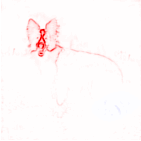
\includegraphics[width=1.5cm]{data/dog_explanation.png}
					};
					
					\draw[color=red!30,{Latex[length=0.2cm, width=0.25cm]}-,line width=0.1cm] (n00) to [out=-10,in=170] (n10) {};
					\draw[color=red!70,{Latex[length=0.2cm, width=0.25cm]}-,line width=0.1cm] (n00) to [out=-20,in=160] (n11) {};
					\draw[color=red!15,{Latex[length=0.2cm, width=0.25cm]}-,line width=0.1cm] (n00) to [out=-30,in=150] (n12) {};
					\draw[color=red!90,{Latex[length=0.2cm, width=0.25cm]}-,line width=0.1cm] (n00) to [out=-40,in=140] (n13) {};
					
					\draw[color=white,{Latex[length=0.2cm, width=0.25cm]}-,line width=0.1cm] (n01) to [out=10,in=190] (n10) {};
					\draw[color=white,{Latex[length=0.2cm, width=0.25cm]}-,line width=0.1cm] (n01) to [out=-10,in=170] (n11) {};
					\draw[color=white,{Latex[length=0.2cm, width=0.25cm]}-,line width=0.1cm] (n01) to [out=-20,in=160] (n12) {};
					\draw[color=white,{Latex[length=0.2cm, width=0.25cm]}-,line width=0.1cm] (n01) to [out=-30,in=150] (n13) {};
					
					\draw[color=red!50,{Latex[length=0.2cm, width=0.25cm]}-,line width=0.1cm] (n02) to [out=20,in=200] (n10) {};
					\draw[color=red!20,{Latex[length=0.2cm, width=0.25cm]}-,line width=0.1cm] (n02) to [out=10,in=190] (n11) {};
					\draw[color=red!15,{Latex[length=0.2cm, width=0.25cm]}-,line width=0.1cm] (n02) to [out=-10,in=170] (n12) {};
					\draw[color=red!75,{Latex[length=0.2cm, width=0.25cm]}-,line width=0.1cm] (n02) to [out=-20,in=160] (n13) {};
					
					\draw[color=white,{Latex[length=0.2cm, width=0.25cm]}-,line width=0.1cm] (n03) to [out=30,in=210] (n10) {};
					\draw[color=white,{Latex[length=0.2cm, width=0.25cm]}-,line width=0.1cm] (n03) to [out=20,in=200] (n11) {};
					\draw[color=white,{Latex[length=0.2cm, width=0.25cm]}-,line width=0.1cm] (n03) to [out=10,in=190] (n12) {};
					\draw[color=white,{Latex[length=0.2cm, width=0.25cm]}-,line width=0.1cm] (n03) to [out=-10,in=170] (n13) {};
					
					\draw[color=red!10,{Latex[length=0.2cm, width=0.25cm]}-,line width=0.1cm] (n04) to [out=40,in=220] (n10) {};
					\draw[color=red!35,{Latex[length=0.2cm, width=0.25cm]}-,line width=0.1cm] (n04) to [out=30,in=210] (n11) {};
					\draw[color=red!50,{Latex[length=0.2cm, width=0.25cm]}-,line width=0.1cm] (n04) to [out=20,in=200] (n12) {};
					\draw[color=red!80,{Latex[length=0.2cm, width=0.25cm]}-,line width=0.1cm] (n04) to [out=10,in=190] (n13) {};
					
					\draw[color=white,{Latex[length=0.2cm, width=0.25cm]}-,line width=0.1cm] (n10) to [out=-10,in=170] (n20) {};
					\draw[color=red!80,{Latex[length=0.2cm, width=0.25cm]}-,line width=0.1cm] (n10) to [out=-20,in=160] (n21) {};
					\draw[color=red!15,{Latex[length=0.2cm, width=0.25cm]}-,line width=0.1cm] (n10) to [out=-30,in=150] (n22) {};
					
					\draw[color=red!35,{Latex[length=0.2cm, width=0.25cm]}-,line width=0.1cm] (n11) to [out=10,in=190] (n20) {};
					\draw[color=red!45,{Latex[length=0.2cm, width=0.25cm]}-,line width=0.1cm] (n11) to [out=-10,in=170] (n21) {};
					\draw[color=red!70,{Latex[length=0.2cm, width=0.25cm]}-,line width=0.1cm] (n11) to [out=-20,in=160] (n22) {};
					
					\draw[color=white,{Latex[length=0.2cm, width=0.25cm]}-,line width=0.1cm] (n12) to [out=20,in=200] (n20) {};
					\draw[color=red!50,{Latex[length=0.2cm, width=0.25cm]}-,line width=0.1cm] (n12) to [out=10,in=190] (n21) {};
					\draw[color=red!95,{Latex[length=0.2cm, width=0.25cm]}-,line width=0.1cm] (n12) to [out=-10,in=170] (n22) {};
					
					\draw[color=red!15,{Latex[length=0.2cm, width=0.25cm]}-,line width=0.1cm] (n13) to [out=30,in=210] (n20) {};
					\draw[color=red!35,{Latex[length=0.2cm, width=0.25cm]}-,line width=0.1cm] (n13) to [out=20,in=200] (n21) {};
					\draw[color=white,{Latex[length=0.2cm, width=0.25cm]}-,line width=0.1cm] (n13) to [out=10,in=190] (n22) {};
					
					\draw[color=red!85,{Latex[length=0.2cm, width=0.25cm]}-,line width=0.1cm] (n20) to [out=-10,in=170] (n31) {};
					
					\draw[color=red!80,{Latex[length=0.2cm, width=0.25cm]}-,line width=0.1cm] (n21) to [out=10,in=190] (n31) {};
					
					\draw[color=red!95,{Latex[length=0.2cm, width=0.25cm]}-,line width=0.1cm] (n22) to [out=20,in=200] (n31) {};
					
				\end{tikzpicture}
			\end{figure}
		\end{center}
	\end{frame}
	

	% LRP cat backward
	\begin{frame}
		\vspace{2.5cm}
		\begin{center}
			\begin{figure}
				\begin{tikzpicture}
					\node[circle,draw=blue!40, fill=blue!40, minimum size=0.65cm, inner sep=2pt] (n00) at (2.5,1.5) {\textcolor{white}{\tiny{-3.1}}};
					\node[circle,draw=white, fill=white, minimum size=0.65cm, inner sep=2pt] (n01) at (2.5,0.75) {};
					\node[circle,draw=blue!65, fill=blue!65, minimum size=0.65cm, inner sep=2pt] (n02) at (2.5,0) {\textcolor{white}{\tiny{-3.8}}};
					\node[circle,draw=white, fill=white, minimum size=0.65cm, inner sep=2pt] (n03) at (2.5,-0.75) {};
					\node[circle,draw=red!30, fill=red!30, minimum size=0.65cm, inner sep=2pt] (n04) at (2.5,-1.5) {\textcolor{white}{\tiny{1.8}}};
					
					\node[circle,draw=blue!35, fill=blue!35, minimum size=0.65cm, inner sep=2pt] (n10) at (4.5,1.125) {\textcolor{white}{\tiny{-2.4}}};
					\node[circle,draw=red!50, fill=red!50, minimum size=0.65cm, inner sep=2pt] (n11) at (4.5,0.375) {\textcolor{white}{\tiny{3.2}}};
					\node[circle,draw=blue!50, fill=blue!50, minimum size=0.65cm, inner sep=2pt] (n12) at (4.5,-0.375) {\textcolor{white}{\tiny{-3.1}}};
					\node[circle,draw=blue!55, fill=blue!55, minimum size=0.65cm, inner sep=2pt] (n13) at (4.5,-1.125) {\textcolor{white}{\tiny{-2.8}}};
					
					\node[circle,draw=blue!45, fill=blue!45, minimum size=0.65cm, inner sep=2pt] (n20) at (6.5,0.75) {\textcolor{white}{\tiny{-3.2}}};
					\node[circle,draw=blue!65, fill=blue!65, minimum size=0.65cm, inner sep=2pt] (n21) at (6.5,0) {\textcolor{white}{\tiny{-3.7}}};
					\node[circle,draw=red!20, fill=red!20, minimum size=0.65cm, inner sep=2pt] (n22) at (6.5,-0.75) {\textcolor{white}{\tiny{1.6}}};
					
					\node[circle,draw=white, fill=white, minimum size=0.65cm, inner sep=2pt, label=right:{\textcolor{white}{\scriptsize{dog}}}] (n31) at (8.5,0.375) {};
					\node[circle,draw=blue!60, fill=blue!60, minimum size=0.65cm, inner sep=2pt, label=right:{\scriptsize{cat}}] (n32) at (8.5,-0.375) {\textcolor{white}{\tiny{-5.1}}};
					
					\draw[color=blue!70,{Latex[length=0.2cm, width=0.25cm]}-,line width=0.1cm] (0.5,0) to [out=0,in=190] (n00) {};
					\draw[color=white,{Latex[length=0.2cm, width=0.25cm]}-,line width=0.1cm] (0.5,0) to [out=0,in=185] (n01) {};
					\draw[color=blue!65,{Latex[length=0.2cm, width=0.25cm]}-,line width=0.1cm] (0.5,0) to [out=0,in=180] (n02) {};
					\draw[color=white,{Latex[length=0.2cm, width=0.25cm]}-,line width=0.1cm] (0.5,0) to [out=0,in=175] (n03) {};
					\draw[color=red!30,{Latex[length=0.2cm, width=0.25cm]}-,line width=0.1cm] (0.5,0) to [out=0,in=170] (n04) {};
	
					\node[inner sep=0pt, draw=black] at (0,0) {
						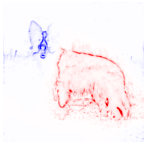
\includegraphics[width=1.5cm]{data/cat_explanation.png}
					};
					
					\draw[color=blue!30,{Latex[length=0.2cm, width=0.25cm]}-,line width=0.1cm] (n00) to [out=-10,in=170] (n10) {};
					\draw[color=red!70,{Latex[length=0.2cm, width=0.25cm]}-,line width=0.1cm] (n00) to [out=-20,in=160] (n11) {};
					\draw[color=blue!15,{Latex[length=0.2cm, width=0.25cm]}-,line width=0.1cm] (n00) to [out=-30,in=150] (n12) {};
					\draw[color=blue!90,{Latex[length=0.2cm, width=0.25cm]}-,line width=0.1cm] (n00) to [out=-40,in=140] (n13) {};
					
					\draw[color=white,{Latex[length=0.2cm, width=0.25cm]}-,line width=0.1cm] (n01) to [out=10,in=190] (n10) {};
					\draw[color=white,{Latex[length=0.2cm, width=0.25cm]}-,line width=0.1cm] (n01) to [out=-10,in=170] (n11) {};
					\draw[color=white,{Latex[length=0.2cm, width=0.25cm]}-,line width=0.1cm] (n01) to [out=-20,in=160] (n12) {};
					\draw[color=white,{Latex[length=0.2cm, width=0.25cm]}-,line width=0.1cm] (n01) to [out=-30,in=150] (n13) {};
					
					\draw[color=blue!50,{Latex[length=0.2cm, width=0.25cm]}-,line width=0.1cm] (n02) to [out=20,in=200] (n10) {};
					\draw[color=red!20,{Latex[length=0.2cm, width=0.25cm]}-,line width=0.1cm] (n02) to [out=10,in=190] (n11) {};
					\draw[color=blue!15,{Latex[length=0.2cm, width=0.25cm]}-,line width=0.1cm] (n02) to [out=-10,in=170] (n12) {};
					\draw[color=blue!75,{Latex[length=0.2cm, width=0.25cm]}-,line width=0.1cm] (n02) to [out=-20,in=160] (n13) {};
					
					\draw[color=white,{Latex[length=0.2cm, width=0.25cm]}-,line width=0.1cm] (n03) to [out=30,in=210] (n10) {};
					\draw[color=white,{Latex[length=0.2cm, width=0.25cm]}-,line width=0.1cm] (n03) to [out=20,in=200] (n11) {};
					\draw[color=white,{Latex[length=0.2cm, width=0.25cm]}-,line width=0.1cm] (n03) to [out=10,in=190] (n12) {};
					\draw[color=white,{Latex[length=0.2cm, width=0.25cm]}-,line width=0.1cm] (n03) to [out=-10,in=170] (n13) {};
					
					\draw[color=blue!10,{Latex[length=0.2cm, width=0.25cm]}-,line width=0.1cm] (n04) to [out=40,in=220] (n10) {};
					\draw[color=red!85,{Latex[length=0.2cm, width=0.25cm]}-,line width=0.1cm] (n04) to [out=30,in=210] (n11) {};
					\draw[color=blue!35,{Latex[length=0.2cm, width=0.25cm]}-,line width=0.1cm] (n04) to [out=20,in=200] (n12) {};
					\draw[color=blue!25,{Latex[length=0.2cm, width=0.25cm]}-,line width=0.1cm] (n04) to [out=10,in=190] (n13) {};
					
					\draw[color=white,{Latex[length=0.2cm, width=0.25cm]}-,line width=0.1cm] (n10) to [out=-10,in=170] (n20) {};
					\draw[color=blue!80,{Latex[length=0.2cm, width=0.25cm]}-,line width=0.1cm] (n10) to [out=-20,in=160] (n21) {};
					\draw[color=red!15,{Latex[length=0.2cm, width=0.25cm]}-,line width=0.1cm] (n10) to [out=-30,in=150] (n22) {};
					
					\draw[color=blue!35,{Latex[length=0.2cm, width=0.25cm]}-,line width=0.1cm] (n11) to [out=10,in=190] (n20) {};
					\draw[color=blue!45,{Latex[length=0.2cm, width=0.25cm]}-,line width=0.1cm] (n11) to [out=-10,in=170] (n21) {};
					\draw[color=red!70,{Latex[length=0.2cm, width=0.25cm]}-,line width=0.1cm] (n11) to [out=-20,in=160] (n22) {};
					
					\draw[color=white,{Latex[length=0.2cm, width=0.25cm]}-,line width=0.1cm] (n12) to [out=20,in=200] (n20) {};
					\draw[color=blue!50,{Latex[length=0.2cm, width=0.25cm]}-,line width=0.1cm] (n12) to [out=10,in=190] (n21) {};
					\draw[color=red!95,{Latex[length=0.2cm, width=0.25cm]}-,line width=0.1cm] (n12) to [out=-10,in=170] (n22) {};
					
					\draw[color=blue!15,{Latex[length=0.2cm, width=0.25cm]}-,line width=0.1cm] (n13) to [out=30,in=210] (n20) {};
					\draw[color=blue!35,{Latex[length=0.2cm, width=0.25cm]}-,line width=0.1cm] (n13) to [out=20,in=200] (n21) {};
					\draw[color=white,{Latex[length=0.2cm, width=0.25cm]}-,line width=0.1cm] (n13) to [out=10,in=190] (n22) {};
					
					\draw[color=blue!45,{Latex[length=0.2cm, width=0.25cm]}-,line width=0.1cm] (n20) to [out=-20,in=160] (n32) {};
					
					\draw[color=blue!65,{Latex[length=0.2cm, width=0.25cm]}-,line width=0.1cm] (n21) to [out=-10,in=170] (n32) {};
					
					\draw[color=red!20,{Latex[length=0.2cm, width=0.25cm]}-,line width=0.1cm] (n22) to [out=10,in=190] (n32) {};
					
				\end{tikzpicture}
			\end{figure}
		\end{center}
	\end{frame}
	
	% LRP cat backward with formula
	\begin{frame}
		\vspace{2.5cm}
		\begin{center}
			\begin{figure}
				\begin{tikzpicture}
					\node[circle,draw=blue!40, fill=blue!40, minimum size=0.65cm, inner sep=2pt] (n00) at (2.5,1.5) {\textcolor{white}{\tiny{-3.1}}};
					\node[circle,draw=white, fill=white, minimum size=0.65cm, inner sep=2pt] (n01) at (2.5,0.75) {};
					\node[circle,draw=blue!65, fill=blue!65, minimum size=0.65cm, inner sep=2pt] (n02) at (2.5,0) {\textcolor{white}{\tiny{-3.8}}};
					\node[circle,draw=white, fill=white, minimum size=0.65cm, inner sep=2pt] (n03) at (2.5,-0.75) {};
					\node[circle,draw=red!30, fill=red!30, minimum size=0.65cm, inner sep=2pt] (n04) at (2.5,-1.5) {\textcolor{white}{\tiny{1.8}}};
					
					\node[circle,draw=blue!35, fill=blue!35, minimum size=0.65cm, inner sep=2pt] (n10) at (4.5,1.125) {\textcolor{white}{\tiny{-2.4}}};
					\node[circle,draw=red!50, fill=red!50, minimum size=0.65cm, inner sep=2pt] (n11) at (4.5,0.375) {\textcolor{white}{\tiny{3.2}}};
					\node[circle,draw=blue!50, fill=blue!50, minimum size=0.65cm, inner sep=2pt] (n12) at (4.5,-0.375) {\textcolor{white}{\tiny{-3.1}}};
					\node[circle,draw=blue!55, fill=blue!55, minimum size=0.65cm, inner sep=2pt] (n13) at (4.5,-1.125) {\textcolor{white}{\tiny{-2.8}}};
					
					\node[circle,draw=blue!45, fill=blue!45, minimum size=0.65cm, inner sep=2pt] (n20) at (6.5,0.75) {\textcolor{white}{\tiny{-3.2}}};
					\node[circle,draw=blue!65, fill=blue!65, minimum size=0.65cm, inner sep=2pt] (n21) at (6.5,0) {\textcolor{white}{\tiny{-3.7}}};
					\node[circle,draw=red!20, fill=red!20, minimum size=0.65cm, inner sep=2pt] (n22) at (6.5,-0.75) {\textcolor{white}{\tiny{1.6}}};
					
					\node[circle,draw=white, fill=white, minimum size=0.65cm, inner sep=2pt, label=right:{\textcolor{white}{\scriptsize{dog}}}] (n31) at (8.5,0.375) {};
					\node[circle,draw=blue!60, fill=blue!60, minimum size=0.65cm, inner sep=2pt, label=right:{\scriptsize{cat}}] (n32) at (8.5,-0.375) {\textcolor{white}{\tiny{-5.1}}};
					
					\draw[color=blue!70,{Latex[length=0.2cm, width=0.25cm]}-,line width=0.1cm] (0.5,0) to [out=0,in=190] (n00) {};
					\draw[color=white,{Latex[length=0.2cm, width=0.25cm]}-,line width=0.1cm] (0.5,0) to [out=0,in=185] (n01) {};
					\draw[color=blue!65,{Latex[length=0.2cm, width=0.25cm]}-,line width=0.1cm] (0.5,0) to [out=0,in=180] (n02) {};
					\draw[color=white,{Latex[length=0.2cm, width=0.25cm]}-,line width=0.1cm] (0.5,0) to [out=0,in=175] (n03) {};
					\draw[color=red!30,{Latex[length=0.2cm, width=0.25cm]}-,line width=0.1cm] (0.5,0) to [out=0,in=170] (n04) {};
	
					\node[inner sep=0pt, draw=black] at (0,0) {
						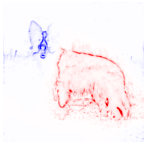
\includegraphics[width=1.5cm]{data/cat_explanation.png}
					};
					\node[inner sep=0pt] at (0,-1.3) {\tiny{$\sum\limits_i R^0_i = -5.1$}};
					
					\draw[color=blue!30,{Latex[length=0.2cm, width=0.25cm]}-,line width=0.1cm] (n00) to [out=-10,in=170] (n10) {};
					\draw[color=red!70,{Latex[length=0.2cm, width=0.25cm]}-,line width=0.1cm] (n00) to [out=-20,in=160] (n11) {};
					\draw[color=blue!15,{Latex[length=0.2cm, width=0.25cm]}-,line width=0.1cm] (n00) to [out=-30,in=150] (n12) {};
					\draw[color=blue!90,{Latex[length=0.2cm, width=0.25cm]}-,line width=0.1cm] (n00) to [out=-40,in=140] (n13) {};
					
					\draw[color=white,{Latex[length=0.2cm, width=0.25cm]}-,line width=0.1cm] (n01) to [out=10,in=190] (n10) {};
					\draw[color=white,{Latex[length=0.2cm, width=0.25cm]}-,line width=0.1cm] (n01) to [out=-10,in=170] (n11) {};
					\draw[color=white,{Latex[length=0.2cm, width=0.25cm]}-,line width=0.1cm] (n01) to [out=-20,in=160] (n12) {};
					\draw[color=white,{Latex[length=0.2cm, width=0.25cm]}-,line width=0.1cm] (n01) to [out=-30,in=150] (n13) {};
					
					\draw[color=blue!50,{Latex[length=0.2cm, width=0.25cm]}-,line width=0.1cm] (n02) to [out=20,in=200] (n10) {};
					\draw[color=red!20,{Latex[length=0.2cm, width=0.25cm]}-,line width=0.1cm] (n02) to [out=10,in=190] (n11) {};
					\draw[color=blue!15,{Latex[length=0.2cm, width=0.25cm]}-,line width=0.1cm] (n02) to [out=-10,in=170] (n12) {};
					\draw[color=blue!75,{Latex[length=0.2cm, width=0.25cm]}-,line width=0.1cm] (n02) to [out=-20,in=160] (n13) {};
					
					\draw[color=white,{Latex[length=0.2cm, width=0.25cm]}-,line width=0.1cm] (n03) to [out=30,in=210] (n10) {};
					\draw[color=white,{Latex[length=0.2cm, width=0.25cm]}-,line width=0.1cm] (n03) to [out=20,in=200] (n11) {};
					\draw[color=white,{Latex[length=0.2cm, width=0.25cm]}-,line width=0.1cm] (n03) to [out=10,in=190] (n12) {};
					\draw[color=white,{Latex[length=0.2cm, width=0.25cm]}-,line width=0.1cm] (n03) to [out=-10,in=170] (n13) {};
					
					\draw[color=blue!10,{Latex[length=0.2cm, width=0.25cm]}-,line width=0.1cm] (n04) to [out=40,in=220] (n10) {};
					\draw[color=red!85,{Latex[length=0.2cm, width=0.25cm]}-,line width=0.1cm] (n04) to [out=30,in=210] (n11) {};
					\draw[color=blue!35,{Latex[length=0.2cm, width=0.25cm]}-,line width=0.1cm] (n04) to [out=20,in=200] (n12) {};
					\draw[color=blue!25,{Latex[length=0.2cm, width=0.25cm]}-,line width=0.1cm] (n04) to [out=10,in=190] (n13) {};
					
					\draw[color=white,{Latex[length=0.2cm, width=0.25cm]}-,line width=0.1cm] (n10) to [out=-10,in=170] (n20) {};
					\draw[color=blue!80,{Latex[length=0.2cm, width=0.25cm]}-,line width=0.1cm] (n10) to [out=-20,in=160] (n21) {};
					\draw[color=red!15,{Latex[length=0.2cm, width=0.25cm]}-,line width=0.1cm] (n10) to [out=-30,in=150] (n22) {};
					
					\draw[color=blue!35,{Latex[length=0.2cm, width=0.25cm]}-,line width=0.1cm] (n11) to [out=10,in=190] (n20) {};
					\draw[color=blue!45,{Latex[length=0.2cm, width=0.25cm]}-,line width=0.1cm] (n11) to [out=-10,in=170] (n21) {};
					\draw[color=red!70,{Latex[length=0.2cm, width=0.25cm]}-,line width=0.1cm] (n11) to [out=-20,in=160] (n22) {};
					
					\draw[color=white,{Latex[length=0.2cm, width=0.25cm]}-,line width=0.1cm] (n12) to [out=20,in=200] (n20) {};
					\draw[color=blue!50,{Latex[length=0.2cm, width=0.25cm]}-,line width=0.1cm] (n12) to [out=10,in=190] (n21) {};
					\draw[color=red!95,{Latex[length=0.2cm, width=0.25cm]}-,line width=0.1cm] (n12) to [out=-10,in=170] (n22) {};
					
					\draw[color=blue!15,{Latex[length=0.2cm, width=0.25cm]}-,line width=0.1cm] (n13) to [out=30,in=210] (n20) {};
					\draw[color=blue!35,{Latex[length=0.2cm, width=0.25cm]}-,line width=0.1cm] (n13) to [out=20,in=200] (n21) {};
					\draw[color=white,{Latex[length=0.2cm, width=0.25cm]}-,line width=0.1cm] (n13) to [out=10,in=190] (n22) {};
					
					\draw[color=blue!45,{Latex[length=0.2cm, width=0.25cm]}-,line width=0.1cm] (n20) to [out=-20,in=160] (n32) {};
					
					\draw[color=blue!65,{Latex[length=0.2cm, width=0.25cm]}-,line width=0.1cm] (n21) to [out=-10,in=170] (n32) {};
					
					\draw[color=red!20,{Latex[length=0.2cm, width=0.25cm]}-,line width=0.1cm] (n22) to [out=10,in=190] (n32) {};
					
				\end{tikzpicture}
			\end{figure}
		\end{center}
	\end{frame}
	
	% SFCN
	\begin{frame}
		\vspace{2.5cm}
		\begin{center}
			\begin{figure}
				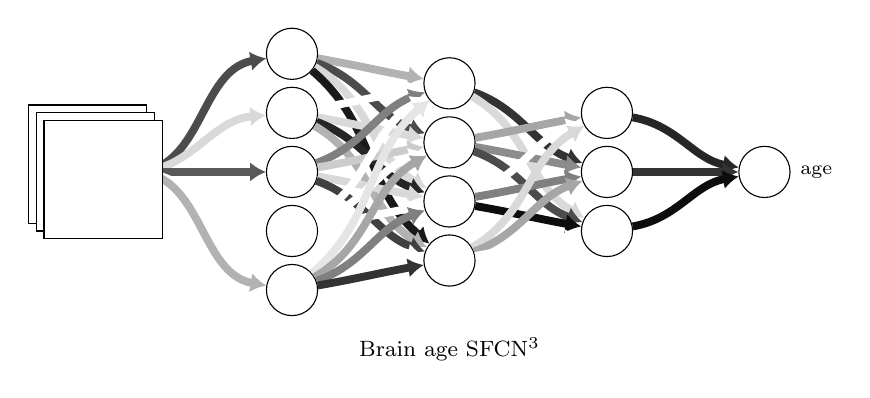
\begin{tikzpicture}
					\node[] at (4.5, -2.25) {\footnotesize{Brain age SFCN\textsuperscript{3}}};
					\node[circle,draw=black, fill=white, minimum size=0.65cm, inner sep=2pt] (n00) at (2.5,1.5) {};
					\node[circle,draw=black, fill=white, minimum size=0.65cm, inner sep=2pt] (n01) at (2.5,0.75) {};
					\node[circle,draw=black, fill=white, minimum size=0.65cm, inner sep=2pt] (n02) at (2.5,0) {};
					\node[circle,draw=black, fill=white, minimum size=0.65cm, inner sep=2pt] (n03) at (2.5,-0.75) {};
					\node[circle,draw=black, fill=white, minimum size=0.65cm, inner sep=2pt] (n04) at (2.5,-1.5) {};
					
					\node[circle,draw=black, fill=white, minimum size=0.65cm, inner sep=2pt] (n10) at (4.5,1.125) {};
					\node[circle,draw=black, fill=white, minimum size=0.65cm, inner sep=2pt] (n11) at (4.5,0.375) {};
					\node[circle,draw=black, fill=white, minimum size=0.65cm, inner sep=2pt] (n12) at (4.5,-0.375) {};
					\node[circle,draw=black, fill=white, minimum size=0.65cm, inner sep=2pt] (n13) at (4.5,-1.125) {};
					
					\node[circle,draw=black, fill=white, minimum size=0.65cm, inner sep=2pt] (n20) at (6.5,0.75) {};
					\node[circle,draw=black, fill=white, minimum size=0.65cm, inner sep=2pt] (n21) at (6.5,0) {};
					\node[circle,draw=black, fill=white, minimum size=0.65cm, inner sep=2pt] (n22) at (6.5,-0.75) {};
					
					\node[circle,draw=black!, fill=white, minimum size=0.65cm, inner sep=2pt, label=right:{\scriptsize{age}}] (n31) at (8.5,0) {};
					
					\draw[color=black!70,-{Latex[length=0.2cm, width=0.25cm]},line width=0.1cm] (0.5,0) to [out=0,in=190] (n00) {};
					\draw[color=black!15,-{Latex[length=0.2cm, width=0.25cm]},line width=0.1cm] (0.5,0) to [out=0,in=185] (n01) {};
					\draw[color=black!65,-{Latex[length=0.2cm, width=0.25cm]},line width=0.1cm] (0.5,0) to [out=0,in=180] (n02) {};
					\draw[color=white,-{Latex[length=0.2cm, width=0.25cm]},line width=0.1cm] (0.5,0) to [out=0,in=175] (n03) {};
					\draw[color=black!30,-{Latex[length=0.2cm, width=0.25cm]},line width=0.1cm] (0.5,0) to [out=0,in=170] (n04) {};
					
					\node[minimum width=1.5cm, minimum height=1.5cm, inner sep=0pt, draw=black, fill=white] at (-0.1,0.1) {};
					\node[minimum width=1.5cm, minimum height=1.5cm, inner sep=0pt, draw=black, fill=white] at (0,0) {};
					\node[minimum width=1.5cm, minimum height=1.5cm, inner sep=0pt, draw=black, fill=white] at (0.1,-0.1) {};
					
					\draw[color=black!30,-{Latex[length=0.2cm, width=0.25cm]},line width=0.1cm] (n00) to [out=-10,in=170] (n10) {};
					\draw[color=black!70,-{Latex[length=0.2cm, width=0.25cm]},line width=0.1cm] (n00) to [out=-20,in=160] (n11) {};
					\draw[color=black!15,-{Latex[length=0.2cm, width=0.25cm]},line width=0.1cm] (n00) to [out=-30,in=150] (n12) {};
					\draw[color=black!90,-{Latex[length=0.2cm, width=0.25cm]},line width=0.1cm] (n00) to [out=-40,in=140] (n13) {};
					
					\draw[color=white,-{Latex[length=0.2cm, width=0.25cm]},line width=0.1cm] (n01) to [out=10,in=190] (n10) {};
					\draw[color=black!15,-{Latex[length=0.2cm, width=0.25cm]},line width=0.1cm] (n01) to [out=-10,in=170] (n11) {};
					\draw[color=black!85,-{Latex[length=0.2cm, width=0.25cm]},line width=0.1cm] (n01) to [out=-20,in=160] (n12) {};
					\draw[color=black!30,-{Latex[length=0.2cm, width=0.25cm]},line width=0.1cm] (n01) to [out=-30,in=150] (n13) {};
					
					\draw[color=black!50,-{Latex[length=0.2cm, width=0.25cm]},line width=0.1cm] (n02) to [out=20,in=200] (n10) {};
					\draw[color=black!20,-{Latex[length=0.2cm, width=0.25cm]},line width=0.1cm] (n02) to [out=10,in=190] (n11) {};
					\draw[color=black!15,-{Latex[length=0.2cm, width=0.25cm]},line width=0.1cm] (n02) to [out=-10,in=170] (n12) {};
					\draw[color=black!75,-{Latex[length=0.2cm, width=0.25cm]},line width=0.1cm] (n02) to [out=-20,in=160] (n13) {};
					
					\draw[color=white,-{Latex[length=0.2cm, width=0.25cm]},line width=0.1cm] (n03) to [out=30,in=210] (n10) {};
					\draw[color=white,-{Latex[length=0.2cm, width=0.25cm]},line width=0.1cm] (n03) to [out=20,in=200] (n11) {};
					\draw[color=white,-{Latex[length=0.2cm, width=0.25cm]},line width=0.1cm] (n03) to [out=10,in=190] (n12) {};
					\draw[color=white,-{Latex[length=0.2cm, width=0.25cm]},line width=0.1cm] (n03) to [out=-10,in=170] (n13) {};
					
					\draw[color=black!10,-{Latex[length=0.2cm, width=0.25cm]},line width=0.1cm] (n04) to [out=40,in=220] (n10) {};
					\draw[color=black!35,-{Latex[length=0.2cm, width=0.25cm]},line width=0.1cm] (n04) to [out=30,in=210] (n11) {};
					\draw[color=black!50,-{Latex[length=0.2cm, width=0.25cm]},line width=0.1cm] (n04) to [out=20,in=200] (n12) {};
					\draw[color=black!80,-{Latex[length=0.2cm, width=0.25cm]},line width=0.1cm] (n04) to [out=10,in=190] (n13) {};
					
					\draw[color=white,-{Latex[length=0.2cm, width=0.25cm]},line width=0.1cm] (n10) to [out=-10,in=170] (n20) {};
					\draw[color=black!80,-{Latex[length=0.2cm, width=0.25cm]},line width=0.1cm] (n10) to [out=-20,in=160] (n21) {};
					\draw[color=black!15,-{Latex[length=0.2cm, width=0.25cm]},line width=0.1cm] (n10) to [out=-30,in=150] (n22) {};
					
					\draw[color=black!35,-{Latex[length=0.2cm, width=0.25cm]},line width=0.1cm] (n11) to [out=10,in=190] (n20) {};
					\draw[color=black!45,-{Latex[length=0.2cm, width=0.25cm]},line width=0.1cm] (n11) to [out=-10,in=170] (n21) {};
					\draw[color=black!70,-{Latex[length=0.2cm, width=0.25cm]},line width=0.1cm] (n11) to [out=-20,in=160] (n22) {};
					
					\draw[color=white,-{Latex[length=0.2cm, width=0.25cm]},line width=0.1cm] (n12) to [out=20,in=200] (n20) {};
					\draw[color=black!50,-{Latex[length=0.2cm, width=0.25cm]},line width=0.1cm] (n12) to [out=10,in=190] (n21) {};
					\draw[color=black!95,-{Latex[length=0.2cm, width=0.25cm]},line width=0.1cm] (n12) to [out=-10,in=170] (n22) {};
					
					\draw[color=black!15,-{Latex[length=0.2cm, width=0.25cm]},line width=0.1cm] (n13) to [out=30,in=210] (n20) {};
					\draw[color=black!35,-{Latex[length=0.2cm, width=0.25cm]},line width=0.1cm] (n13) to [out=20,in=200] (n21) {};
					\draw[color=white,-{Latex[length=0.2cm, width=0.25cm]},line width=0.1cm] (n13) to [out=10,in=190] (n22) {};
					
					\draw[color=black!85,-{Latex[length=0.2cm, width=0.25cm]},line width=0.1cm] (n20) to [out=-10,in=170] (n31) {};
					
					\draw[color=black!80,-{Latex[length=0.2cm, width=0.25cm]},line width=0.1cm] (n21) to (n31) {};
					
					\draw[color=black!95,-{Latex[length=0.2cm, width=0.25cm]},line width=0.1cm] (n22) to [out=10,in=190] (n31) {};
					
				\end{tikzpicture}
			\end{figure}
		\end{center}
	\end{frame}
	
	% Brain age forward
	\begin{frame}
		\vspace{2.5cm}
		\begin{center}
			\begin{figure}
				\begin{tikzpicture}					
					\node[circle,draw=black!70, fill=black!70, minimum size=0.65cm, inner sep=2pt] (n00) at (2.5,1.5) {\textcolor{white}{\tiny{0.70}}};
					\node[circle,draw=black!15, fill=black!15, minimum size=0.65cm, inner sep=2pt] (n01) at (2.5,0.75) {\tiny{0.15}};
					\node[circle,draw=black!65, fill=black!65, minimum size=0.65cm, inner sep=2pt] (n02) at (2.5,0) {\textcolor{white}{\tiny{0.65}}};
					\node[circle,draw=white, fill=white, minimum size=0.65cm, inner sep=2pt] (n03) at (2.5,-0.75) {};
					\node[circle,draw=black!30, fill=black!30, minimum size=0.65cm, inner sep=2pt] (n04) at (2.5,-1.5) {\tiny{0.30}};
					
					\node[circle,draw=black!35, fill=black!35, minimum size=0.65cm, inner sep=2pt] (n10) at (4.5,1.125) {\tiny{0.35}};
					\node[circle,draw=black!20, fill=black!20, minimum size=0.65cm, inner sep=2pt] (n11) at (4.5,0.375) {\tiny{0.20}};
					\node[circle,draw=black!40, fill=black!40, minimum size=0.65cm, inner sep=2pt] (n12) at (4.5,-0.375) {\tiny{0.40}};
					\node[circle,draw=black!85, fill=black!85, minimum size=0.65cm, inner sep=2pt] (n13) at (4.5,-1.125) {\textcolor{white}{\tiny{0.85}}};
					
					\node[circle,draw=black!10, fill=black!10, minimum size=0.65cm, inner sep=2pt] (n20) at (6.5,0.75) {\tiny{0.10}};
					\node[circle,draw=black!95, fill=black!95, minimum size=0.65cm, inner sep=2pt] (n21) at (6.5,0) {\textcolor{white}{\tiny{0.95}}};
					\node[circle,draw=black!70, fill=black!70, minimum size=0.65cm, inner sep=2pt] (n22) at (6.5,-0.75) {\textcolor{white}{\tiny{0.70}}};
					
					\node[circle,draw=black!45, fill=black!45, minimum size=0.65cm, inner sep=2pt, label=right:{\scriptsize{age}}] (n31) at (8.5,0) {\textcolor{white}{\tiny{37.0}}};
					
					\draw[color=black!70,-{Latex[length=0.2cm, width=0.25cm]},line width=0.1cm] (0.5,0) to [out=0,in=190] (n00) {};
					\draw[color=black!15,-{Latex[length=0.2cm, width=0.25cm]},line width=0.1cm] (0.5,0) to [out=0,in=185] (n01) {};
					\draw[color=black!65,-{Latex[length=0.2cm, width=0.25cm]},line width=0.1cm] (0.5,0) to [out=0,in=180] (n02) {};
					\draw[color=white,-{Latex[length=0.2cm, width=0.25cm]},line width=0.1cm] (0.5,0) to [out=0,in=175] (n03) {};
					\draw[color=black!30,-{Latex[length=0.2cm, width=0.25cm]},line width=0.1cm] (0.5,0) to [out=0,in=170] (n04) {};
					
					\node[minimum width=1.5cm, minimum height=1.5cm, inner sep=0pt, draw=black, fill=black] at (-0.1,0.1) {
						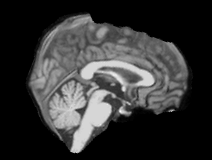
\includegraphics[width=1.5cm]{data/slice.png}
					};
					\node[minimum width=1.5cm, minimum height=1.5cm, inner sep=0pt, draw=black, fill=black] at (0,0) {
						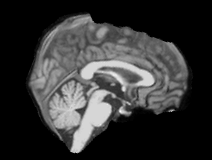
\includegraphics[width=1.5cm]{data/slice.png}
					};
					\node[minimum width=1.5cm, minimum height=1.5cm, inner sep=0pt, draw=black, fill=black] at (0.1,-0.1) {
						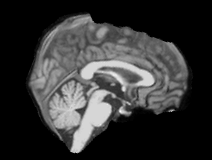
\includegraphics[width=1.5cm]{data/slice.png}
					};
					
					\draw[color=black!30,-{Latex[length=0.2cm, width=0.25cm]},line width=0.1cm] (n00) to [out=-10,in=170] (n10) {};
					\draw[color=black!70,-{Latex[length=0.2cm, width=0.25cm]},line width=0.1cm] (n00) to [out=-20,in=160] (n11) {};
					\draw[color=black!15,-{Latex[length=0.2cm, width=0.25cm]},line width=0.1cm] (n00) to [out=-30,in=150] (n12) {};
					\draw[color=black!90,-{Latex[length=0.2cm, width=0.25cm]},line width=0.1cm] (n00) to [out=-40,in=140] (n13) {};
					
					\draw[color=white,-{Latex[length=0.2cm, width=0.25cm]},line width=0.1cm] (n01) to [out=10,in=190] (n10) {};
					\draw[color=black!15,-{Latex[length=0.2cm, width=0.25cm]},line width=0.1cm] (n01) to [out=-10,in=170] (n11) {};
					\draw[color=black!85,-{Latex[length=0.2cm, width=0.25cm]},line width=0.1cm] (n01) to [out=-20,in=160] (n12) {};
					\draw[color=black!30,-{Latex[length=0.2cm, width=0.25cm]},line width=0.1cm] (n01) to [out=-30,in=150] (n13) {};
					
					\draw[color=black!50,-{Latex[length=0.2cm, width=0.25cm]},line width=0.1cm] (n02) to [out=20,in=200] (n10) {};
					\draw[color=black!20,-{Latex[length=0.2cm, width=0.25cm]},line width=0.1cm] (n02) to [out=10,in=190] (n11) {};
					\draw[color=black!15,-{Latex[length=0.2cm, width=0.25cm]},line width=0.1cm] (n02) to [out=-10,in=170] (n12) {};
					\draw[color=black!75,-{Latex[length=0.2cm, width=0.25cm]},line width=0.1cm] (n02) to [out=-20,in=160] (n13) {};
					
					\draw[color=white,-{Latex[length=0.2cm, width=0.25cm]},line width=0.1cm] (n03) to [out=30,in=210] (n10) {};
					\draw[color=white,-{Latex[length=0.2cm, width=0.25cm]},line width=0.1cm] (n03) to [out=20,in=200] (n11) {};
					\draw[color=white,-{Latex[length=0.2cm, width=0.25cm]},line width=0.1cm] (n03) to [out=10,in=190] (n12) {};
					\draw[color=white,-{Latex[length=0.2cm, width=0.25cm]},line width=0.1cm] (n03) to [out=-10,in=170] (n13) {};
					
					\draw[color=black!10,-{Latex[length=0.2cm, width=0.25cm]},line width=0.1cm] (n04) to [out=40,in=220] (n10) {};
					\draw[color=black!35,-{Latex[length=0.2cm, width=0.25cm]},line width=0.1cm] (n04) to [out=30,in=210] (n11) {};
					\draw[color=black!50,-{Latex[length=0.2cm, width=0.25cm]},line width=0.1cm] (n04) to [out=20,in=200] (n12) {};
					\draw[color=black!80,-{Latex[length=0.2cm, width=0.25cm]},line width=0.1cm] (n04) to [out=10,in=190] (n13) {};
					
					\draw[color=white,-{Latex[length=0.2cm, width=0.25cm]},line width=0.1cm] (n10) to [out=-10,in=170] (n20) {};
					\draw[color=black!80,-{Latex[length=0.2cm, width=0.25cm]},line width=0.1cm] (n10) to [out=-20,in=160] (n21) {};
					\draw[color=black!15,-{Latex[length=0.2cm, width=0.25cm]},line width=0.1cm] (n10) to [out=-30,in=150] (n22) {};
					
					\draw[color=black!35,-{Latex[length=0.2cm, width=0.25cm]},line width=0.1cm] (n11) to [out=10,in=190] (n20) {};
					\draw[color=black!45,-{Latex[length=0.2cm, width=0.25cm]},line width=0.1cm] (n11) to [out=-10,in=170] (n21) {};
					\draw[color=black!70,-{Latex[length=0.2cm, width=0.25cm]},line width=0.1cm] (n11) to [out=-20,in=160] (n22) {};
					
					\draw[color=white,-{Latex[length=0.2cm, width=0.25cm]},line width=0.1cm] (n12) to [out=20,in=200] (n20) {};
					\draw[color=black!50,-{Latex[length=0.2cm, width=0.25cm]},line width=0.1cm] (n12) to [out=10,in=190] (n21) {};
					\draw[color=black!95,-{Latex[length=0.2cm, width=0.25cm]},line width=0.1cm] (n12) to [out=-10,in=170] (n22) {};
					
					\draw[color=black!15,-{Latex[length=0.2cm, width=0.25cm]},line width=0.1cm] (n13) to [out=30,in=210] (n20) {};
					\draw[color=black!35,-{Latex[length=0.2cm, width=0.25cm]},line width=0.1cm] (n13) to [out=20,in=200] (n21) {};
					\draw[color=white,-{Latex[length=0.2cm, width=0.25cm]},line width=0.1cm] (n13) to [out=10,in=190] (n22) {};
					
					\draw[color=black!85,-{Latex[length=0.2cm, width=0.25cm]},line width=0.1cm] (n20) to [out=-10,in=170] (n31) {};
					
					\draw[color=black!80,-{Latex[length=0.2cm, width=0.25cm]},line width=0.1cm] (n21) to (n31) {};
					
					\draw[color=black!95,-{Latex[length=0.2cm, width=0.25cm]},line width=0.1cm] (n22) to [out=10,in=190] (n31) {};
					
				\end{tikzpicture}
			\end{figure}
		\end{center}
	\end{frame}
	
	% Brain age backward
	\begin{frame}
		\vspace{2.5cm}
		\begin{center}
			\begin{figure}
				\begin{tikzpicture}					
					\node[circle,draw=red!70, fill=red!70, minimum size=0.65cm, inner sep=2pt] (n00) at (2.5,1.5) {\textcolor{white}{\tiny{16.0}}};
					\node[circle,draw=white, fill=white, minimum size=0.65cm, inner sep=2pt] (n01) at (2.5,0.75) {};
					\node[circle,draw=red!65, fill=red!65, minimum size=0.65cm, inner sep=2pt] (n02) at (2.5,0) {\textcolor{white}{\tiny{13.0}}};
					\node[circle,draw=white, fill=white, minimum size=0.65cm, inner sep=2pt] (n03) at (2.5,-0.75) {};
					\node[circle,draw=red!30, fill=red!30, minimum size=0.65cm, inner sep=2pt] (n04) at (2.5,-1.5) {\textcolor{white}{\tiny{8.0}}};
					
					\node[circle,draw=red!35, fill=red!35, minimum size=0.65cm, inner sep=2pt] (n10) at (4.5,1.125) {\textcolor{white}{\tiny{7.0}}};
					\node[circle,draw=red!40, fill=red!40, minimum size=0.65cm, inner sep=2pt] (n11) at (4.5,0.375) {\textcolor{white}{\tiny{8.0}}};
					\node[circle,draw=red!50, fill=red!50, minimum size=0.65cm, inner sep=2pt] (n12) at (4.5,-0.375) {\textcolor{white}{\tiny{9.0}}};
					\node[circle,draw=red!35, fill=red!35, minimum size=0.65cm, inner sep=2pt] (n13) at (4.5,-1.125) {\textcolor{white}{\tiny{5.0}}};
					
					\node[circle,draw=red!20, fill=red!20, minimum size=0.65cm, inner sep=2pt] (n20) at (6.5,0.75) {\textcolor{white}{\tiny{7.0}}};
					\node[circle,draw=red!95, fill=red!95, minimum size=0.65cm, inner sep=2pt] (n21) at (6.5,0) {\textcolor{white}{\tiny{19.0}}};
					\node[circle,draw=red!70, fill=red!70, minimum size=0.65cm, inner sep=2pt] (n22) at (6.5,-0.75) {\textcolor{white}{\tiny{11.0}}};
					
					\node[circle,draw=red!80, fill=red!80, minimum size=0.65cm, inner sep=2pt, label=right:{\scriptsize{age}}] (n31) at (8.5,0) {\textcolor{white}{\tiny{37.0}}};
					
					\draw[color=red!70,{Latex[length=0.2cm, width=0.25cm]}-,line width=0.1cm] (0.5,0) to [out=0,in=190] (n00) {};
					\draw[color=white,{Latex[length=0.2cm, width=0.25cm]}-,line width=0.1cm] (0.5,0) to [out=0,in=185] (n01) {};
					\draw[color=red!65,{Latex[length=0.2cm, width=0.25cm]}-,line width=0.1cm] (0.5,0) to [out=0,in=180] (n02) {};
					\draw[color=white,{Latex[length=0.2cm, width=0.25cm]}-,line width=0.1cm] (0.5,0) to [out=0,in=175] (n03) {};
					\draw[color=red!30,{Latex[length=0.2cm, width=0.25cm]}-,line width=0.1cm] (0.5,0) to [out=0,in=170] (n04) {};
	
					\node[minimum width=1.5cm, minimum height=1.5cm, inner sep=0pt, draw=black, fill=white] at (-0.1,0.1) {
						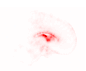
\includegraphics[width=1.48cm]{data/brain_age_explanation.png}
					};
					\node[minimum width=1.5cm, minimum height=1.5cm, inner sep=0pt, draw=black, fill=white] at (0,0) {
						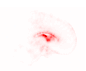
\includegraphics[width=1.48cm]{data/brain_age_explanation.png}
					};
					\node[minimum width=1.5cm, minimum height=1.5cm, inner sep=0pt, draw=black, fill=white] at (0.1,-0.1) {
						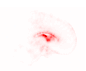
\includegraphics[width=1.48cm]{data/brain_age_explanation.png}
					};
					
					\draw[color=red!30,{Latex[length=0.2cm, width=0.25cm]}-,line width=0.1cm] (n00) to [out=-10,in=170] (n10) {};
					\draw[color=red!70,{Latex[length=0.2cm, width=0.25cm]}-,line width=0.1cm] (n00) to [out=-20,in=160] (n11) {};
					\draw[color=red!15,{Latex[length=0.2cm, width=0.25cm]}-,line width=0.1cm] (n00) to [out=-30,in=150] (n12) {};
					\draw[color=red!90,{Latex[length=0.2cm, width=0.25cm]}-,line width=0.1cm] (n00) to [out=-40,in=140] (n13) {};
					
					\draw[color=white,{Latex[length=0.2cm, width=0.25cm]}-,line width=0.1cm] (n01) to [out=10,in=190] (n10) {};
					\draw[color=white,{Latex[length=0.2cm, width=0.25cm]}-,line width=0.1cm] (n01) to [out=-10,in=170] (n11) {};
					\draw[color=white,{Latex[length=0.2cm, width=0.25cm]}-,line width=0.1cm] (n01) to [out=-20,in=160] (n12) {};
					\draw[color=white,{Latex[length=0.2cm, width=0.25cm]}-,line width=0.1cm] (n01) to [out=-30,in=150] (n13) {};
					
					\draw[color=red!50,{Latex[length=0.2cm, width=0.25cm]}-,line width=0.1cm] (n02) to [out=20,in=200] (n10) {};
					\draw[color=red!20,{Latex[length=0.2cm, width=0.25cm]}-,line width=0.1cm] (n02) to [out=10,in=190] (n11) {};
					\draw[color=red!15,{Latex[length=0.2cm, width=0.25cm]}-,line width=0.1cm] (n02) to [out=-10,in=170] (n12) {};
					\draw[color=red!75,{Latex[length=0.2cm, width=0.25cm]}-,line width=0.1cm] (n02) to [out=-20,in=160] (n13) {};
					
					\draw[color=white,{Latex[length=0.2cm, width=0.25cm]}-,line width=0.1cm] (n03) to [out=30,in=210] (n10) {};
					\draw[color=white,{Latex[length=0.2cm, width=0.25cm]}-,line width=0.1cm] (n03) to [out=20,in=200] (n11) {};
					\draw[color=white,{Latex[length=0.2cm, width=0.25cm]}-,line width=0.1cm] (n03) to [out=10,in=190] (n12) {};
					\draw[color=white,{Latex[length=0.2cm, width=0.25cm]}-,line width=0.1cm] (n03) to [out=-10,in=170] (n13) {};
					
					\draw[color=red!10,{Latex[length=0.2cm, width=0.25cm]}-,line width=0.1cm] (n04) to [out=40,in=220] (n10) {};
					\draw[color=red!35,{Latex[length=0.2cm, width=0.25cm]}-,line width=0.1cm] (n04) to [out=30,in=210] (n11) {};
					\draw[color=red!50,{Latex[length=0.2cm, width=0.25cm]}-,line width=0.1cm] (n04) to [out=20,in=200] (n12) {};
					\draw[color=red!80,{Latex[length=0.2cm, width=0.25cm]}-,line width=0.1cm] (n04) to [out=10,in=190] (n13) {};
					
					\draw[color=white,{Latex[length=0.2cm, width=0.25cm]}-,line width=0.1cm] (n10) to [out=-10,in=170] (n20) {};
					\draw[color=red!80,{Latex[length=0.2cm, width=0.25cm]}-,line width=0.1cm] (n10) to [out=-20,in=160] (n21) {};
					\draw[color=red!15,{Latex[length=0.2cm, width=0.25cm]}-,line width=0.1cm] (n10) to [out=-30,in=150] (n22) {};
					
					\draw[color=red!35,{Latex[length=0.2cm, width=0.25cm]}-,line width=0.1cm] (n11) to [out=10,in=190] (n20) {};
					\draw[color=red!45,{Latex[length=0.2cm, width=0.25cm]}-,line width=0.1cm] (n11) to [out=-10,in=170] (n21) {};
					\draw[color=red!70,{Latex[length=0.2cm, width=0.25cm]}-,line width=0.1cm] (n11) to [out=-20,in=160] (n22) {};
					
					\draw[color=white,{Latex[length=0.2cm, width=0.25cm]}-,line width=0.1cm] (n12) to [out=20,in=200] (n20) {};
					\draw[color=red!50,{Latex[length=0.2cm, width=0.25cm]}-,line width=0.1cm] (n12) to [out=10,in=190] (n21) {};
					\draw[color=red!95,{Latex[length=0.2cm, width=0.25cm]}-,line width=0.1cm] (n12) to [out=-10,in=170] (n22) {};
					
					\draw[color=red!15,{Latex[length=0.2cm, width=0.25cm]}-,line width=0.1cm] (n13) to [out=30,in=210] (n20) {};
					\draw[color=red!35,{Latex[length=0.2cm, width=0.25cm]}-,line width=0.1cm] (n13) to [out=20,in=200] (n21) {};
					\draw[color=white,{Latex[length=0.2cm, width=0.25cm]}-,line width=0.1cm] (n13) to [out=10,in=190] (n22) {};
					
					\draw[color=red!85,{Latex[length=0.2cm, width=0.25cm]}-,line width=0.1cm] (n20) to [out=-10,in=170] (n31) {};
					
					\draw[color=red!80,{Latex[length=0.2cm, width=0.25cm]}-,line width=0.1cm] (n21) to  (n31) {};
					
					\draw[color=red!95,{Latex[length=0.2cm, width=0.25cm]}-,line width=0.1cm] (n22) to [out=10,in=190] (n31) {};
					
				\end{tikzpicture}
			\end{figure}
		\end{center}
	\end{frame}

	% Brain age LRP gif
	\begin{frame}
	\end{frame}
\end{document}
